\documentclass{report}
%Math Stuff
\usepackage{amsmath}
\usepackage{enumitem}
\usepackage{mathtools}

%General Formating
\usepackage[letterpaper, portrait, margin=1in]{geometry}
\usepackage{fancyhdr}
\pagestyle{fancy}

%Bibliography
\usepackage[toc,page]{appendix}
\usepackage{hyperref}

%Figures
\usepackage{graphicx}
\graphicspath{ {figures/} }
\usepackage{tikz}
\usepackage{pgfmath}
\usepackage{framed}
\usepackage{csvsimple}
\usepackage{rotating}
\usepackage[section]{placeins}

%Header
\lhead{Schulman}
\rhead{Page \thepage}

%Title
\title{Food Networks \\~\\ \normalsize A Thesis Presented to the Faculty of the Economics Department of Cornell University in Partial Fulfillment of the Requirements for the Degree of Bachelor of Arts in Economics with Honors} 
\author{Eric Schulman}
\date{May 2017}

\begin{document}

\maketitle

\pagebreak

\begin{abstract}
For my thesis, I ask how the network of farms, intermediaries, and stores involved with agricultural production relates to prices and consumer behavior. Suppliers face transportation costs while navigating products from farms to stores. Estimating these costs might provide insight into the prices consumers face at stores. To estimate transportation costs in the network, I track the supply of grapes, cabbage, onions, and cherries as it moves from farms to stores in New York state using data from satellites and public records. Using this data, I estimate the least costly path for transporting the goods from the farms to the stores using a linear programming software package. According to my estimates, transporting produce to northeast and southeastern parts of the state is most expensive. Additionally, when the farms vary in size, the cost of sending produce to stores gets noticeably amplified in the optimal solution. All of the code to used to complete this project is publicly available on GitHub at \url{http://github.com/erichschulman/ag_networks}. 
\end{abstract}

\pagebreak

\renewcommand{\abstractname}{Acknowledgments}
\begin{abstract}
This has been an incredible experience and I've learned so much! I couldn't have done this project without the tremendous amount of support I've gotten from the faculty in the department of economics. I want to explicitly thank Professor Patacchini for advising the project and Professor Besharov for running the honors program. I also want to thank Professor Tardos in computer science for helping me to understand the algorithms involved with this project and Professor Easley and Professor Caunedo for their feedback over the past few months. 
\end{abstract}

\tableofcontents

%background
\chapter{Introduction}
\section{Background}

Economics and nutrition are no strangers. Economists and other social scientists have been measuring nutritional outcomes for years. The literature calls adequate nutritional outcomes 'food security'. Food security consists of three dimensions: availability, accessibility, and utilization. Availability reflects whether food is available in stores. Access reflects whether people can afford it. Utilization reflects what people do with food after buying it \cite{barrett}. In the past, researchers measured food security using a questionnaire about nutritional practices. The questionnaire asks respondents whether they purchased vegetables, ate 3 meals each day, or similar questions. Responses to the questionnaire reflects levels of food security.

For a long time, researchers have explained the answers to surveys about food security using their statistical relationship with transfer programs and demographics. The United States publishes a survey about food security each month called the CPS nutritional supplement. Demographic information about participants in the nutritional supplement gets tracked as part of the regular CPS so calculating the statistical relationships between the survey and factors like race, income, and education is relatively easy.

This literature finds that reducing costs and increasing availability of nutritional foods improves health outcomes. One study evaluated the Farmers' Market Nutrition Program, a national program intended to increase consumption of fresh fruits and vegetables by providing coupons and information. Researchers found subsidizing nutritionally rich food with coupons leads to increased consumption when complemented with information \cite{Just}. As it developed, the literature began noticing the importance of systemic factors in determining nutritional outcomes. For example, researchers analyzed nutritional outcomes in Oregon between 1999 and 2001, when Oregon had the highest average rate of hunger in the nation. The study found factors like residential location and housing costs were most related to food insecurity \cite{Bernell}.

In recent years, social scientists interested in nutrition have shifted towards looking at nutrition habits in the context of people's environments, thinking of people as part of a food network. Instead of trying to measure the statistical relationship between a family or individual characteristics with their eating outcomes, the researchers classify environments that put individuals at risk to be unhealthy. Most studies call areas where residents have difficulty maintaining a balanced diet 'food deserts'. The term originated to describe public housing developments in western Scotland with a limited number of grocery stores and other options for nutritious foods. Especially in the past 5 years, this term has captured the imagination of policy makers in the United States.

A lot of research has been focused on finding and classifying food deserts or areas. These studies leverage spatial coordinates and mapping software to classify areas based on their risk for being food insecure using their proximity to grocers and markets. Often times, these studies augment their observations using demographic information.  One study conducted among grocery stores across inner cities and suburbs within the Minneapolis and St. Paul metropolitan concluded the urban poor pay marginally more for food because supermarket chains don't open in inner cities \cite{Chung}. Researchers began applying the label "food deserts" to inner cities. With more data becoming available online, researchers continue describing food supply in more detail to understand systemic food insecurity. In one project, researchers leveraged Google Maps, and local online news to build a graphical representation of food availability in Bogota, Columbia \cite{Hwang}. Another study used online directories of grocery stores to index neighborhoods' vulnerability to food insecurity in the twin cities area \cite{Larson}.

The literature on food deserts focuses on observing the locations of food suppliers. It generally ignores the endogenous factors that determine the placement of stores even though researchers in the field of operations research have studied how suppliers decide on the allocation of food. Food allocation is often studied using a transportation problem. Transportation problems are an optimization problem designed to find the cheapest possible way of sending a certain amount of supply through a network. A typical application of this problem involves finding the best delivery route from a factory to a warehouse where the road network has some capacity and cost associated. Solving the problem involves finding a vector with an economic interpretation of optimal prices from a social planning perspective. It can be solved efficiently using the network simplex algorithm and linear programming software packages \cite{Cook}. Researchers often apply transportation problems to food allocation. One paper studies maize allocation in south Africa where trains carry maize from supply and demand points, scattered throughout the country. Researchers minimize the total rail cost, as is standard, but add a secondary objective of distributing costs fairly among all users \cite{Stewart}.

\section{Research Question} 

For my project, I ask what areas of New York state make purchasing fresh produce expensive due to their position in the network of farms, stores and intermediaries. Following much of the nascent literature on food deserts, I use spatial data and demographic information to identify regions where obtaining produce is difficult for structural reasons.

I improve the literature identifying food deserts in two ways. Most studies do not comment on whether people rural areas can easily access nutritional food. Most studies, identify food deserts using detailed directories of stores and calculating residents proximity to those stores. These records do not exists for rural areas meaning rural areas are often overlooked by the literature. More importantly, using the distances between people and stores to identify areas where people do not have nutritional food ignores the endogenous factors that determine where stores get built and how prices get set. My project, considers prices in rural areas and endogenous factors into account by focusing my analysis to a few crops and leveraging the operations research literature regarding the optimal allocation of food. For my project, I estimate the prices for onions, cherries, grapes, and cabbages across New York state using information about the supply chain.

Although I expand my analysis to encapsulate the endogenous factor involved with supply, my study falls like most of the literature on food deserts. due to time constraints, availability of data, and the complexity of the problem, I ignore data regarding consumer behavior in classifying areas regarding the ease of finding produce. Still, most of the literature does not even acknowledge this shortcoming and modeling supply takes a step in the right direction. Also, the estimates I made are interesting in themselves. By estimating costs in the transportation network, certain observation about how the distribution of farms and stores effects costs emerge. Additionally, the literature finds a statistical relationship between high prices and worse outcomes. These observations could be useful in further focusing the scope of future investigations that include consumer behavior.

\section{Economic Mechanism}

In order to predict where produce was expensive, I tracked the supply chain of cherries, cabbages, and onions come in New York state using satellite data and public records. I used this data to estimate the cost of moving the produce from farms to stores. Since, the crops I chose are not produced on a large scale transportation costs are a good indicator of prices. The factors involved with production are similar so transportation costs are the main difference in the costs faced by suppliers. By shifting the supply curve out for certain suppliers, transportation costs main are the main difference in prices. This means that the transportation costs have serious weight in terms of predicting which areas it is difficult to get fresh produce.

Focusing on crops with a shorter shelf life makes tracking their supply chain relatively simple. With the exception of grapes, production of these crops is limited as you can see from Table \ref{tab:nass3}. For this reason, It largely falls into three stages. First, farms produce crops. Then they send their goods to intermediaries called agricultural dealers. The agricultural dealers may do some intermediate processing (like putting to produce in bags), but they largely leave the produce alone. The facilitate the movement of produce between farms and stores. After agricultural dealers send the produce to stores who in turn allow consumers to buy the crop.  Cabbage, onions and cherries have relatively short shelf lives discouraging the crops from being sold out of state. As you can see, in Table \ref{tab:nass2}. This table compares production of these crops to the amount of these crops that are sold for USDA organic crops \cite{nass2}.

New York releases data on the size and location of farms, the locations of the agricultural dealers, and the size and locations of stores. Since the crops are sent directly from farms to dealers to stores, I  have a snapshot of the crops at each stage through their production. It seems reasonable to assume farms move their goods through the state in such a way that satisfies demand, but keeps costs as low as possible. Building on the assumption that farms, dealers, and stores try to minimize the of moving produce through the network, I can fill in the missing pieces to estimate how produce dynamically moves through the state. In this way, my project incorporates the literature of looking at agricultural markets as an optimization problem by optimizing the transportation costs through this network based on the produces' initial and final locations.

\begin{table}
\centering
\begin{framed}
\begin{tabular}{c|c|c|c}%
	Item&Sales (1000 USD)&Rank by Sales&Percent of Total Sales
    \csvreader[head to column names]{nass3.csv}{}% use head of csv as column names
    {\\\hline \csvcoli & \csvcolii & \csvcoliii & \csvcoliv}
\end{tabular}
\caption{This table shows various crops in New York state. Fresh produce (i.e. Fruits and Vegetables) makes up about $10 \%$ of New York's agricultural sales \cite{nass3}.}
\label{tab:nass3}
\end{framed}
\end{table}


\begin{table}
\centering
\begin{framed}
\begin{tabular}{c|c|c|c|c}%
	Crop&Total Production (CWT)& Fresh Market Sales (CWT)&Percentage&Year
    \csvreader[head to column names]{nass2.csv}{}% use head of csv as column names
    {\\\hline \csvcoli & \csvcolii & \csvcoliii & \csvcoliv& \csvcolv}
\end{tabular}
\caption{This table compares the organic production of the various bands of crops in New York to the amount that is sold on the fresh market \cite{nass2}. The amount produced and sold is measured in hundredweight (CWT). About 17 CWT make up a US ton. I chose 2011 as the year because that was the year the crop cover data was produced. There are few things to note in this table. The these crops are USDA organic meaning that they don't represent all production. Organic cherries are produced in such limited quantity in New York that their production isn't included in the data.}
\label{tab:nass2}
\end{framed}
\end{table}

\chapter{Linear Model}

\section{Model Overview}

The optimization problem of minimizing costs while meeting demand is called optimal transportation. It is also called minimum-cost flow. It tries to maximize the amount of flow (in my case units of produce flowing through the network of farms, stores, and intermediaries) at the minimum cost.  Minimum-cost flow is a more general version of a matching market. For my project, I apply this frame work to agricultural markets in New York to understand how the network is related to costs. I have the snap-shot of a network. In the network, Farms can ship to any intermediary associated with the same crop and intermediaries can ship to any store. Intermediaries can scale as much as they desire. Farms produce agricultural products proportional to their size. Although I do not have the exact amount of produce sold by stores, it seems reasonable to assume it would be proportional to the cost of their square footage. This costs represents the majority of the stores fixed cost. By modeling these crops using this framework, I fill in the missing details of my snapshot about how the produce is moving through the network.

To solve the problem, you can start by maximizing the amount of goods you've sent through the network without worrying about cost.  After finding the maximum amount of goods flowing through the network, you find try to optimize cost.  If you are familiar with matching markets and augmenting paths, this problem will look familiar. You start by using augmenting paths to find the maximum amount of flow through the network. Then you try to optimize its cost by finding a reduced cost path. A reduced cost path works exactly like an augmenting path in a matching market but instead of increasing the amount of goods, you try to reduce the costs while keeping the amount of goods constant. You start at a supply node and trace a path alternating between supply and demand until you reach your original node while reducing cost. If you can trace back to your initial node then you've reduced the cost. You repeat this process until you've exhausted all of the reduced cost cycles. To get a better sense of the problem and how to  solve it, I worked out a  manageable example of a transportation problem with a network of 2 suppliers and 3 consumers in Figures \ref{fig:example1} through \ref{fig:example6}. Following the example makes the nature of the problem and how to solve it significantly more clear. Understanding the problem in the abstract much more complicated than a concrete example.

Because I had a lot of variables to solve for I solved this problem as linear and used the simplex algorithm (as opposed the the algorithm in Figures \ref{fig:example1} through \ref{fig:example6}). The algorithm finds the solution to a linear objective (i.e. $a x_1 +b x_2 + ...$ ) subjected to linear constraints. The intuition behind how it works involves solving the problem in two ways to finds the lowest maximum and highest minimum. When these coincide,  you know you found a maximum.

Using the simplex algorithm to solve my problem is efficient. Measuring a program's efficiency using factors like how long it takes to run or how many lines of code it takes can vary with the computer, the compiler and the input to the program. As a result, in order to have a more universal measure of efficiency the efficiency of algorithms are measured using run time bounds. Run time bounds are an upper bound on the number of steps you need to solve the problem, given the input's size.  The simplex algorithm's run time bound is bad as far as we know. It can be $O(2^n)$. Meaning that if there could be some scalar multiple of $2^n$ steps if there are $n$ input variables. However, in practice the simplex algorithm does much better. The general rule of thumb is that the simplex algorithm has a run time bound that is some polynomial of $n$ \cite{Cook}.

At first glance, the  linear nature of the problem function might look like OLS. The problems have mathematical similarities. However, practically speaking they are used differently. Generally speaking, OLS produces estimates parameters that are interesting in a statistical sense.  The parameters in linear programming are more interesting as point values. They are interesting purely because they satisfies the objective function. Perhaps measuring transportation costs in this way is a foolish way to look at the data. However, the more I explore the data, the more doubtful I am that a statistical model could capture the intricate relationships between farmers, intermediaries and stores across the state. As opposed to looking at statstical properties, the linear program tries to formally describe the mechanism that firms use to decide the transportation costs.

Since  open source code is important, I've made all the code I wrote for this project publicly available on GitHub with a detailed explanation about how to get it running. It's mostly written in python, with a few SQL queries. Since open source is important to me, most of the software dependencies that need to be installed in order to get my code working are open source. The one exception is the linear optimizer. In this case, I used Gurobi for which an academic license is free. You can access the code at \url{http://github.com/erichschulman/ag_networks}.

\section{Primal Problem}

In order to use linear programming packages, we need to formally state the problem as a linear program in a way the computer can understand. As we said before, the problem tries to send as much units of a good from a suppliers $s$ in the set $S$ to consumers $d$ in the set $D$. However, there are costs for sending a unit of good across every route between suppliers and consumers. We want to minimize these costs which leads to our objective function (in the objective $c$ is costs and $u$ is units of the good). 

$$\operatorname{Minimize} \sum_{s,d \in \text{Routes}} c_{s,d} u_{s,d}$$

The constraints on the objective function reflect the fact that supply and demand must should balance. The first set of constraints require that demand be satisfied.

$$\sum_{s,d \in \text{Routes}} \text{u}_{s,d}= \text{demand at } d \text{ (for all consumers } s \in S)$$

The second set of constraint requires that no supply goes to waste. In other words, no product is just left at suppliers. In this case, supply is a negative quantity because supply leaves the supply nodes and flows to demand nodes.

$$\sum_{s,d \in \text{Routes}} \text{u}_{s,d}= \text{supply at } s \text{ (for all suppliers } d \in D)$$

Finally, we can't have negative amounts of units flow across the routes.

$$0 \leq u_{s,d},  \text{ for all edges } s,d \in \text{Routes}$$

Putting it all together, supply in demand balance because suppliers are required to send a certain amount of flow and consumers must receive a certain amount.
$$\operatorname{Minimize} \sum_{s,d \in \text{Routes}} c_{s,d} u_{s,d}$$
$$\text{subject to}$$
$$\sum_{s,d \in \text{Routes}} \text{u}_{s,d}= \text{demand at } d \text{ (for all suppliers } s \in S)$$
$$\sum_{s,d \in \text{Routes}} \text{u}_{s,d}= \text{supply at } s \text{ (for all consumers } d \in D)$$
$$0 \leq u_{s,d}, \text{ for all edges } s,d \in \text{Routes}$$

To summarize, the objective function minimizes total costs. The first and second constraints ensure nodes either produce or consume based on their type; the third ensures supply moves forward from supply to demand.  In the case, when supply does not equal demand you can add an extra node to the problem. You let other nodes send supply or receive goods from this node at 0 cost (depending on whether there is too much supply or demand). The amount flow from this node to others represents a shortage or surplus.

%reduction

The network I'm looking at is slightly more complicated than just supply and demand nodes though. I drew a picture of how I modified the transportation network in Figure \ref{fig:spec}. Assuming I can measure demand, supply, and the edge costs in the network, I can reduce the problem I've described to optimal transportation. By reduce, I mean I want to show that the problem I specified above can be  written as a linear program which I can solve with the simplex algorithm. In this section, I will be formally explaining the way I did this. It is easy to see this linear program for my agricultural networks is  the same as minimum cost flow. Farms are suppliers and stores are consumers. Supplies and demands balance because these crops are not really exported. The only difference is the inclusion of processors. Farms can send produce to which ever processor they like and processors can send produce to which ever store they like. However, farms cannot send their produce straight to the stores. The objective function is updated to reflect this change. Farms must incur the cost of sending their goods to processors, and stores incur the cost of receiving their goods from processors (instead of just sending goods between farms and stores like the original problem).

$$\operatorname{Minimize} \sum_{f,p \in \text{Routes}} c_{f,p} u_{f,p} + \sum_{p,s \in \text{Routes}} c_{p,s} u_{p,s}$$

We also need to add an additional constraint onto the processors in the linear program. This constraint prevents the processors from keeping any of the crops.

$$\sum_{f,p \in \text{Routes}} \text{u}_{f,p} + \sum_{p,s \in \text{Routes}} \text{u}_{p,s} = 0 \text{ (for all processors } p \in P)$$

So, putting ething together we specify the primal problem:

$$\operatorname{Minimize} \sum_{f,p \in \text{Routes}} c_{f,p} u_{f,p} + \sum_{p,s \in \text{Routes}} c_{p,s} u_{p,s}$$
$$\text{subject to}$$
$$\sum_{f,p \in \text{Routes}} \text{u}_{f,p}= \text{supply at } f \text{ (for all farms } f \in F)$$
$$\sum_{f,p \in \text{Routes}} \text{u}_{f,p} + \sum_{p,s \in \text{Routes}} \text{u}_{p,s} = 0 \text{ (for all processors } p \in P)$$
$$\sum_{p,s \in \text{Routes}} \text{u}_{p,s}= \text{demand at } s \text{ (for all stores } s \in S)$$
$$0 \leq u_{s,d}, \text{ for all edges } s,d \in \text{Routes}$$

So to summarize, we are minimizing the cost of sending goods from farms to processors and processors to stores. In the problem, we are imposing the constraints that farms send all the crops they grow, stores consume all the crops they receive and processors do not keep any crops. This is  optimal transport.

%dual problem
\section{Dual Problem}

Every linear problem can be stated two different ways as a "primal" and "dual" problem. In the dual version of a linear program the constraints become the variables of interest in a new objective function and old variables become the new constraints. An intuitive way to think about the dual problem is that you find a maximum from all possible minimums in the primal problem. In other words, you try to push the value of the original constraints as high as possible while maintaining the structure of the original primal problem. I just described the "primal" version of optimal transport. I will now state the second, "dual" way of looking at it because it is more relevant to my project. I used the dual problem to solve optimal transport because it yields a more interesting economic interpretation. The dual variables can be interpreted as the optimal prices that incentivize firms to send their goods along the optimal path. If the dual prices at a node are high, that means it is costly to send goods to that node. Instead of finding the amount of units sent between each pair of suppliers and consumers, we can look prices that reflect the relative cost of sending goods to certain parts of the network.

The intuition behind the dual problem for optimal transport comes from the desire to get rid of reduced cost cycles (i.e. paths through the network who's total cost is negative). The dual formalizes this idea. To build the dual problem, you introduce a slack variable called $p$ at each node. In other words, when you compute the costs of a cycle through the network by adding up the costs of each edge in the cycle, you add and subtract $p$ at each node. Adding $p$ does not change how costly the cycle was because as long as the slack variables cancel out you are just left with the cost of traveling through cycle.

Since $p$ is a slack variable, it can take what ever value you want. For our objective function we abritrarily let the difference between $p_d$ (i.e. $p$ at a demand node $d$) and $p_s$  (i.e. $p$ at a supplier $s$) represent the amount you can reduce the costs of a cycle by sending a unit of good from $p$ to $d$. In order to reduce the costs of cylces as much as possible, we want to maximize the value of $p_d - p_s$ for all of the nodes.  In order to complete our objective function, we need to account for the fact multiple units will be sent from $s$ to $d$. Multiple units of flow can be sent accross each edge. To account for the fact that certain nodes are visited more than once, you scale the prices at each node. The amount you scale the prices is equal to the amount of product they will be recieving or sending (i.e. the net flow). It helps to think of the dual variable as a price. You are maximizing the difference revenue of selling the good at $d$ and buying the good at $s$. From here we have enough to write our objective.

$$\operatorname{Maximize} \sum_{d \in D}  (\text{demand at } d) \cdot p_{d} -   \sum_{s \in S}  (\text{supply at } s) \cdot p_{s} $$

The constraints in the dual variable reflect the fact that you can only reduce the cost across an edge so much. At a certain point, you must incur some cost for traversing an edge. The most you can reduce the cost of traversing from from supplier $s$ to demand $d$ is the edge cost between the two $c_{s,d}$. Again, it helps to think of the dual variable as a price. Firms $s$ earns $p_d$ for sending their product to $d$ but looses $p_s + c_{s,w}$. The constraint prevents arbitrage through the network.  The constraints say that the price at the source plus the edge cost must outweigh the cost at the destination.

$$ p_d -p_s  \leq c_{s,d}$$

So, putting it all together we have formalized our dual problem

$$\operatorname{Maximize} \sum_{d \in D}  (\text{demand at } d) \cdot p_{d} -   \sum_{s \in S}  (\text{supply at } s) \cdot p_{s} $$
$$ \text{ subject to}$$
$$ -p_s + p_d \leq c_{s,d},  \text{ for all edges }  s,d\in \textrm{Routes}$$

%reduction
Of course as before, we have to modify the problem to reflect the inclusion of intermediaries. The dual problem's objective stays exactly the same as before because the netflow through the intermediate processors is 0.

$$\operatorname{Maximize} \sum_{s \in S}  (\text{demand at } s) \cdot p_{s} -   \sum_{f \in F}  (\text{supply at } f) \cdot p_{f} $$

Since, we've added processors into the primal's objective function we now need two sets of constraints, one to reflect to cost of sending goods from farms to processors, and another for the cost of sending goods between the processors and stores. These restrictions  prevent every farm from sending their goods to a certain processor and processors from sending all their goods to a certain store.

$$ -p_f + p_p \leq c_{f,p}, \text{ for all edges }  f,p\in \textrm{Routes}$$
$$ -p_p + p_s \leq c_{p,s}, \text{ for all edges }  p,s\in \textrm{Routes}$$

Putting ething together we have our dual problem:

$$\operatorname{Maximize} \sum_{s \in S}  (\text{demand at } s) \cdot p_{s} -   \sum_{f \in F}  (\text{supply at } f) \cdot p_{f} $$
$$ \text{ subject to}$$
$$ -p_f + p_p \leq c_{f,p}, \text{ for all edges } f,p\in \textrm{Routes}$$
$$ -p_p + p_s \leq c_{p,s}, \text{ for all edges } p,s\in \textrm{Routes}$$

\chapter{Data Sources}

\section{Overview}

\section{Farms}

I am in the unqiue position where I can estimate transportation costs using the linear program because of the agriculutral datasets New York state makes publically available. Using New York's data you can track the supply chain of crops who's movements are simple. In my picture of supply, farm's production is proportional to their area. Since, I chose a fairly small geographic region soil, weather, and other elements that effect the production of a crop will not vary greatly. Unless farmers have access to drastically different technologies, the biggest difference affecting yields for farms is the area they've dedicated to growing the crop. I can figure out each farms area by looking at an image created by the National Agricultural Statistical Service \cite{nass}.

I use the pixels in a satellite image of crop cover to see supply. The data set is called the Cropland Data Layer and is created by measuring the way light reflects off the Earth at certain wavelengths using a satellite called Landsat. The satellite measures this reflection at $30 \times 30$ square meter plots. Based on the reflection is possible to classify point measured by the satellite. The classifications are made using training data from the Farm Service Agency Common Land Unit Program and non-agricultural training data from the United States Geological Survey National Land Cover Dataset 2001. The file forms a grid called a raster. Pixels in the image represent certain crop bands. The accuracy of classification for these pixels isn't great. In Table \ref{tab:band}, you can see how accurate the satellite data is.

Although individual pixels may be unreliable, I am counting on the fact that clusters of pixels do  correspond to the locations of farms. Since, I was interested in the area taken up by farms, I used a technique called sieving to make the image more uniform and get rid of random pixels. this technique involves identifying clusters of continuous pixels and dropping the pixels in clusters smaller than a certain size. After creating the sieve, I converted the raster file into vector based polygons to calculate the area of each cluster and the centroid. Each cluster of continuous pixels became a farm with an area and a centroid. to visualize what farms looked like across the various bands I've included Figure \ref{tab:farms}. You can see how farms for each band look (and how an explanation of how the shapes related to the results) in the results section.

\begin{table}
\centering
\begin{framed}
\begin{tabular}{c|c|c|c|c|c}%
	Crop&Band&Correct Pixels&Producer's Accuracy&Kappa&User's Accuracy
    \csvreader[head to column names]{band.csv}{}% use head of csv as column names
    {\\\hline \csvcoli & \csvcolii & \csvcoliii & \csvcoliv& \csvcolv & \csvcolvi}
\end{tabular}
\caption{This table shows the various errors associated with pixels in each crop band in the satellite image \cite{nass}. The pixels are compared with a small test set for accuracy. Correct pixels are the number of pixels extrapolated from the training data. Producer's accuracy is a false negative, where pixels of a known class are classified as something other than that class. User's accuracy shows false positives, where pixels are incorrectly classified as a known class when they should have been classified as something else. Kappa index of agreement gives an overall assessment of the accuracy of the classification.}
\label{tab:band}
\end{framed}
\end{table}


\begin{table}
\centering
\begin{framed}
\begin{tabular}{c|c|c|c|c|c}%
	Crop&Total Area&Average&Minimum&Maximum&Variance
    \csvreader[head to column names]{farms.csv}{}% use head of csv as column names
    {\\\hline \csvcoli & \csvcolii & \csvcoliii & \csvcoliv& \csvcolv & \csvcolvi}
\end{tabular}
\caption{This table is meant to summarize some statistics of interest about the size of farms. The areas are measured in square-meters. Some take aways are that onions (band 49) take up the most area followed by grapes (band 69). Cabbages (band 243) have the smallest range of sizes, but the highest variance within that range. Cherries (band 66) have the smallest variance and the smallest total cover.}
\label{tab:farms}
\end{framed}
\end{table}

\section{Agricultural Dealers}

I included the intermediate processors in the problem for two reasons. They make the problem more realistic because generally farms do not sell their product directly to stores rather intermediaries.  More over, produce is not exported or drastically changed during intermediate processing. If the crops make it to these dealers they are going to be sold to stores then consumed in state. Only 2 of the 300 dealers registered with teh state where out of state. The produce is not altered because you need additional permits for purposes other than resale.  the dealers can sell it to businesses that make prepared foods but in practice, the business with the necessary permits for processing also buy in bulk directly from farms. 

The second reason for including the dealers is because they number of edges to make the problem more computationally tractable. There were roughly 300 licensed agricultural product dealers in the data set. By forcing the edges between stores and farms to the processors, I drastically cut down the number of edges. 

In order to include intermediate processors (i.e. the agricultural product dealers) into the problem, I used the data on permits from the NYS Department of Agricultural Markets \cite{dam}. The state keeps a list of all the businesses that buy more than 10,000 dollars in agricultural products. The data set had information about the crops they sold, and their location as an address. I converted the addresses to a spatial coordinate using Nominatim, an open source platform for geolocating (i.e. converting addresses into coordinates). There are roughly 300 of them, but only half were relevant to my problem because they sold the right type of crop. I've included Table \ref{tab:procs} to visualize how many processors were associated with each crop band. I do not have capacities on the agricultural dealers. It seems reasonable to say the dealers can scale to accept as much product as stores want to send.

\begin{table}
\centering
\begin{framed}
\begin{tabular}{c|c}%
	Crop & Count
    \csvreader[head to column names]{procs.csv}{}% use head of csv as column names
    {\\\hline \csvcoli & \csvcolii}
\end{tabular}
\caption{Grapes (band 69) has the highest number of intermediaries associated with it. The lowest is cherries (band 66).}
\label{tab:procs}
\end{framed}
\end{table}

%stores
\section{Stores}

I cannot see the exact amount of produce sold by stores in New York. Since, Cabbages, cherries, and onions production in New York mostly satisfies in state demand because of these crops' relatively shorter shelf life a smaller scale production, I assume that the amount of produce in the state does not change from farms to stores. 

I also assume the amount of goods sold at a store would be proportional to its size weighted by property values. This is because I imagine stores preform an optimization problem when choosing how much square footage to buy for their store. If square footage is expensive, it reflects that fact that this location is more lucrative to the store. If stores could have higher turn over on inexpensive plots, I would imagine the price would rise. This is by no means precise; just a better estimate of capacity than just square footage. Intuitively, the median housing prices reflects the fact that a stores might have smaller square footage but similar demand. Stores in New York City might be the same size as a store upstate, but sell significantly more produce because the population density is much tighter in New York City and the consumers have more income to spend.  

Another reason for using the weighted size reflects the fact that the amount a store sells is proportional to its fixed costs. Higher fixed costs mean the grocery stores need to sell more to recoup their investment. Although I do not have the exact fixed costs I can approximate the cost of their property by multiplying size by median property values. The cost of the property makes up the majority of a stores fixed cost.

The data I used on stores came from NYS Division of Food Safety. It is the list of stores that are given health inspections. The store data set has roughly 20,000 different stores, the classifications are based on their permits, their square footage, and their location (as a GPS coordinate). I choose to look at the classification 'JAC' which are vendors that are registered as stores, manufacturers and multiple operations. This is because grocery stores fall under this category. Other categories were not as common and less relevant to selling fresh produce. I've included a map to give a sense of how they are spread through out the state in Figure \ref{fig:map_3}. To get a sense of how the stores vary in size, I've included Table \ref{tab:stores}.

So as not to have too many edges between the stores and the intermediaries, I aggregated the number of edges by Census tract. The reason for using this method to aggregate stores reflects the fact that median property values only measured at this level of granularity. Also, the census tracts for the most part represent municipalities. Two stores in the same town probably face the same demand for produce. You can see these weights in Figure \ref{fig:map_4}.


\begin{table}
\centering
\begin{framed}
\begin{tabular}{c|c|c|c}%
	Average&Minimum&Maximum&Variance
    \csvreader[head to column names]{stores.csv}{}% use head of csv as column names
    {\\\hline \csvcoli & \csvcolii & \csvcoliii & \csvcoliv}
\end{tabular}
\caption{This table conveys summary statistics about the characteristics of stores' square footage. Each of the columns are measured in square footage}
\label{tab:stores}
\end{framed}
\end{table}



\section{Edge Costs}

I edges between each farm and processor, and each processor and store. To measure the cost of moving the produce between farms, dealers and stores, I combine open source, publicly available maps of New York state's roads with open source routing software. The cost of traversing edge are expected travel time measured in seconds. 

For the crops I chose, travel times are an adequate measure of costs. These crops are grown on a small scale so roads are the best method for transporting the produce. The other factors involved with transporting produce like fuel, vehicle size, and wages to drivers are standard across the state. Additionally, the crops I analyze are being transported short enough distances in small enough quantities that I do not have to worry about a non-linear cost structure involved with transportation.

The open source software I use to measure travel times is called open source routing machine (OSRM). The algorithm that OSRM implements is called contraction hierarchies. It is a technique to speed up shortest-path routing by first creating precomputed "contracted" versions of the connection graph. Contraction hierarchies can be used to generate shortest-path routes much more efficiently than the standard shortest path algorithm (i.e. Dijkstra's shortest path algorithm).

I downloaded a map of New York from the open source mapping project (OSM) and answered routing queries over my local network about routing. I included two tables to visualize the summary statistics of the edges. Table \ref{tab:fp_edges} shows the average, minimum, maximum, and variance of edges between farms and product dealers. Table \ref{tab:ps_edges} shows the same for the edges between dealers and stores.


\begin{table}[!htb]
\centering
\begin{framed}
\begin{tabular}{c|c|c|c|c}%
	Crop&Average&Minimum&Maximum&Variance
    \csvreader[head to column names]{fp_edges.csv}{}% use head of csv as column names
    {\\\hline \csvcoli & \csvcolii & \csvcoliii & \csvcoliv & \csvcolv}
\end{tabular}
\caption{This table conveys summary statistics about the characteristics of the edges between farms and agricultural product dealers. Grapes (band 69) have the highest variability between edges. Each of the columns is measured in seconds of expected travel time}
\label{tab:fp_edges}
\end{framed}
\end{table}


\begin{table}[!htb]
\centering
\begin{framed}
\begin{tabular}{c|c|c|c|c}%
	Crop&Average&Minimum&Maximum&Variance
    \csvreader[head to column names]{ps_edges.csv}{}% use head of csv as column names
    {\\\hline \csvcoli & \csvcolii & \csvcoliii & \csvcoliv & \csvcolv}
\end{tabular}
\caption{This table conveys summary statistics about the characteristics of the edges between farms and agricultural product dealers. The distances are relatively similar to those of between farms and processors, but they are less variable. Each of the columns is measured in seconds of expected travel time. }
\label{tab:ps_edges}
\end{framed}
\end{table}

\chapter{Results}

\section{Overview}

For my project, I asked how the network of farms, agricultural dealers, and store related with transportation prices. To find out, I tracked the movements of certain crops and estimated the cost by optimizing the movement of the crops. The estimate assigns a cost to each part of the network. This means, that farms, stores and processors all get a price. It seems reasonable to assume these transportation prices are highly related to actual prices based on the structure of the network. By seeing which regions have the highest transportation prices, you can get a much better sense of how to direct future inquiries about how the network and consequently transportation prices effect prices. 

The most interesting part of the problem is the prices at the store nodes. As you would expect, these estimates a lot to do with the concentration of stores, house prices, and the locations of farms. If you are curious about the locations of stores and the and median house prices, you can see them Figures \ref{fig:map_3} and Figure \ref{fig:map_4}. The farm and processor nodes also get prices. The prices at the farms and prices result when multiple stores are competing to receive resources from this node. For example, if a farm with a limited capacity is next to a lot of stores, you need to increase the price at that farm. This makes it less attractive for the nearby stores to ship produce from that farm.

According to the estimates, prices in western part of the state are relatively low at stores. This happened because farms are located in this regions and the median house prices are relatively low. There is a lot of supply and little demand.  On the other hand, the south east and the northern corners of the state are significantly higher at stores. The south east faces the highest prices. This is unsurprising. Property values in this area are high and the concentration of farms is low. That the north would also be high in price was more surprising. Property values are low enough in this region to facilitate farming.  Prices are high here because the agricultural activities that take place are mostly focused on corn and dairy. The farms growing produce are also farthest from the state's northern regions. This is a troubling observation especially when you consider that this region also has some of the lower median incomes in the state. 

You might be wondering why solving the optimization problem was necessary. It seems obvious that your distance from farms and property vales would increase prices for fresh produce. Using the linear program to estimate prices is more tangible and formal way to combine these separate of New York agriculture describe and quantify them. By estimating prices in the transportation network, certain observation about how the distribution of farms and stores effects costs emerge. It turns out that less obvious properties of the network can effect transportation prices. 

Specifically, more farms smaller in size reduce the variance in relative costs through out the state. This finding is highly related to the structure of the linear program. When you have fewer big farms, stores face bigger difference when choosing between farms. If the closest farm does not have enough capacity for all the nearby stores, then stores are forced to chose a farm that is further away incurring higher costs. When the farms are smaller, the difference between the closest farm and the second closest is more gradual. As a result, the difference in prices for the various stores is less pronounced. I noticed this effect in New York state data because it occurs in  prices for onion farms. The farms are smaller and evenly distributed. As a result, the solution looks different than the other bands. Additionally, variance in the sizes of farms gets amplified by the linear program. For example, in the cabbage band variance among the size of farms results in huge disparities in prices.

\section{Visualizing Results}

Understanding over all trends in the linear program isn't obvious. It outputs a list of roughly 8000 prices. In order to glean the key trends, I created tables that summarize key statistics about the linear program's result. Table \ref{tab:county_49}, Table \ref{tab:county_66}, Table \ref{tab:county_69}, and Table \ref{tab:county_243} all summarize the range of possible prices in the linear program for each of the crop bands I analyze. These tables also summarize what county has the highest and lowest prices. As I said before, the counties in the west tend to have the lowest prices. The counties in the south east tend to have the highest prices, followed by the north. The key take aways are that farms are in the western part of the state, but there is a cluster in the southern part of the state. As a result, prices according to the linear program should be cheapest in these places. Prices are most expensive in the northeast corner of the state, followed by the southeast (i.e. Long Island). Again I want to qualify these statements about prices by saying that prices only represent relative transportation prices. Table  \ref{tab:price_49}, Table  \ref{tab:price_66}, Table  \ref{tab:price_69}, and Table  \ref{tab:price_243} all show basic summary statistics about the mean, and variance of the prices in the linear program solution.

I also visualized the solution to the optimization problem over a map of New York state to make the nature of the network for each crop and the result of the linear program intelligible. The first the images shows the locations of farms based on the crop cover data that was put through the sieve. When you look at the pictures of farms, it becomes obvious how they influenced the solution. Areas around the farms have lower prices. Additionally, the differences in the solutions are explained mostly by the differences in the distribution of the farms throughout the state because  the stores and for the most part dealers stay the same between the various bands in the problem. Figure \ref{fig:farms_49}, Figure \ref{fig:farms_66}, Figure \ref{fig:farms_69}, and Figure \ref{fig:farms_243} show the location of farms for each of the respective crop bands.

The second map I created for each band shows the locations of the farms, stores and dealers on the same map. This is just meant to give a sense of what the network looks like. Farms are represented by pentagons, dealers are stars, and stores are squares. Figure \ref{fig:network_49} , Figure \ref{fig:network_66} , Figure \ref{fig:network_69} , and Figure \ref{fig:network_243} all show how the network looks for each of the respective bands. The final image I created for each band is the most interesting as it  visualizes the results of the linear program. It shows the various census tracts with shading based on the relative magnitude of the prices. The  number assigned to the price is some what irrelevant because they only have meaning in relation to each other. They prices reflect the extra time spent on transportation due to including each tract in the network. They are  relative costs due to transportation. Figure \ref{fig:prices_49} , Figure \ref{fig:prices_66} , Figure \ref{fig:prices_69} , and Figure \ref{fig:prices_243} all show how the network looks for each of the respective bands.

\section{Comparing Crop Bands}

There were differences between the results for each of the different crops. Onion prices are unique because there was a cluster of farms in the southern part of the state caused prices to be lower there compared to some of the other bands. Onions have both the lowest prices and the lowest variance among prices do to how spread out they are along the state. Stores are not competing with each other to import onions from the same farm. More over, the farms are relatively close by.

In terms of the various bands Cherries are by far the smallest band in terms of the amount that are sold. Their production is focused in the western portion of the state. Prices are cheapest by farms and most expensive at the southeastern and northeastern parts of the state. The fact that their production is so small and seasonal leads me to question the accuracy of this band. 

The grape farms are concentrated in the southwestern part of the state. There are some farms in the center of the state and also eastern Long Island. I included this section because I calculated the edge costs for the grape farms which takes a long time. I don't think that grapes  are traded using this framework. The supply grown at farms is mostly turned into juices and wines.

Cabbages ended up being the most visually interesting band. For most of the state, the result looks the same as the rest of the state. However, because of the variance in farms, price are much higher in the south east. The variance in the prices calculated is noticeably higher than any of the other bands as we can see in Table \ref{tab:price_243}. This result is more striking in Figure \ref{fig:prices_243}. This result is directly related to the location of the farms through out the state. This is the detail that changes the most between crop bands. Although cabbages are also farmed in the western portion of the state, they are more spread apart and their size is more variable. This result translates through the network creating huge disparities the further away from the farms you go.

I also provided Table \ref{tab:farm_price} to compare the prices for farms, Table \ref{tab:proc_price} to compare the prices for processors, and Table \ref{tab:store_price} to compare the prices for the various census tracts in each of the bands. Table \ref{tab:farm_county}, Table \ref{tab:proc_county}, and Table \ref{tab:store_county} to compare the information on minimum and maximum counties between the band for farms, dealers and stores.

I also included three images comparing the prices generated at the intermediaries by the linear program for cabbages to onions, cherries, and grapes in Figures \ref{fig:procs_243_49}, Figures \ref{fig:procs_243_66}, and Figures \ref{fig:procs_243_69}. Similarly, I've also included three images comparing the prices generated at the census tracts by the linear program for cabbages to onions, cherries, and grapes in Figures \ref{fig:stores_243_49}, Figures \ref{fig:stores_243_66}, and Figures \ref{fig:stores_243_69}.


%%%%%%%%%%%%%%%%%%%%%%%%%%%%%%%%%%%%%%%%%%%%%%%%%%%%%%%%%%%%%%%%%
%Descriptive Statistics 1 %%%%%%%%%%%%%%%%%%%%%%%%%%%%%%%%%%%%%%%
%%%%%%%%%%%%%%%%%%%%%%%%%%%%%%%%%%%%%%%%%%%%%%%%%%%%%%%%%%%%%%%%%


\begin{table}
\centering
\begin{framed}
\begin{tabular}{c|c|c|c}%
	Crop&Average&Variance&Deviation
    \csvreader[head to column names]{price_49.csv}{}% use head of csv as column names
    {\\\hline \csvcoli & \csvcolii & \csvcoliii & \csvcoliv}
\end{tabular}
\caption{This table shows descriptive statistics about the prices in the linear program  for onions as measured in added travel time. The prices from the program represent added travel time in seconds. You can see that the farms in the onion band are spread out enough that the program did not need to increase the price at the farms. The prices at farms and processors get raised when multiple stores compete to buy onions from the same store.}
\label{tab:price_49}
\end{framed}
\end{table}

\begin{table}
\centering
\begin{framed}
\begin{tabular}{c|c|c|c}%
	Crop&Average&Variance&Deviation
    \csvreader[head to column names]{price_66.csv}{}% use head of csv as column names
    {\\\hline \csvcoli & \csvcolii & \csvcoliii & \csvcoliv}
\end{tabular}
\caption{This table shows descriptive statistics about the prices in the linear program for cherries as measured in added travel time. The cherry farms are small enough and spread apart enough that stores do not have to compete between sources. Stores can buy cherries from their most preferred farm. As a result, the price at farms is zero for all farms. Since there are less agricultural dealers that sell cherries and the farms are further from stores, the average price is higher then compared to the other bands.}
\label{tab:price_66}
\end{framed}
\end{table}

\begin{table}
\centering
\begin{framed}
\begin{tabular}{c|c|c|c}%
	Crop&Average&Variance&Deviation
    \csvreader[head to column names]{price_69.csv}{}% use head of csv as column names
    {\\\hline \csvcoli & \csvcolii & \csvcoliii & \csvcoliv}
\end{tabular}
\caption{This table shows descriptive statistics about the prices in the linear program as measured in added travel time for grapes. You can see prices at farms are relatively low, meaning farms are spread far enough apart so that stores do not have to compete over where to buy from. Variance in prices are high for this band.}
\label{tab:price_69}
\end{framed}
\end{table}

\begin{table}
\centering
\begin{framed}
\begin{tabular}{c|c|c|c}%
	Crop&Average&Variance&Deviation
    \csvreader[head to column names]{price_243.csv}{}% use head of csv as column names
    {\\\hline \csvcoli & \csvcolii & \csvcoliii & \csvcoliv}
\end{tabular}
\caption{This table shows descriptive statistics about the prices in the linear program as measured in added travel time for cabbages. The variance of the prices is much lower than the other bands. Additionally, the cabbages are more expensive in the southeast in relatively affluent areas. In the other bands, the crops were more expensive in the northwest. }
\label{tab:price_243}
\end{framed}
\end{table}

%%%%%%%%%%%%%%%%%%%aggregate%%%%%%%%%%%%%%%%%%%%%%%%%%%


\begin{table}
\centering
\begin{framed}
\begin{tabular}{c|c|c|c}%
	Crop&Average&Variance&Deviation
    \csvreader[head to column names]{farm_price.csv}{}% use head of csv as column names
    {\\\hline \csvcoli & \csvcolii & \csvcoliii & \csvcoliv}
\end{tabular}
\caption{This table compares the various prices for the different farm bands in one place as measured in expected travel time.  The prices at farms are non-zero at farms at the center of the network to encourage stores to ship produce from more remote farms. Prices are lowest at the cherry farms, as they are zero.This means that stores are not requesting cherries from the same farm.  The next lowest prices are at onion farms. Prices have the highest variance form the cabbage farms meaning certain farms are very popular with stores. There are more cabbage farms spread out over the western portion of the state. This means that all the eastern stores want to import produce from the central counties (Onondaga). As a result, the price needs to be increased to disincentive stores from ordering produce from these farms.}
\label{tab:farm_price}
\end{framed}
\end{table}


\begin{table}
\centering
\begin{framed}
\begin{tabular}{c|c|c|c}%
	Crop&Average&Variance&Deviation
    \csvreader[head to column names]{proc_price.csv}{}% use head of csv as column names
    {\\\hline \csvcoli & \csvcolii & \csvcoliii & \csvcoliv}
\end{tabular}
\caption{This table compares the prices for the different agricultural dealers across the four bands in one place as measured in expected travel time. Cabbages have the highest price reflecting the similarly high price at farms. The prices at the dealers reflects prices at farms. Cabbages have high prices at dealers reflecting the westward spread of farms.  Grapes have the highest variance reflecting the dense distribution of farms on the southwestern part of the state. Processors in this region have similarly disparate prices when compared }
\label{tab:proc_price}
\end{framed}
\end{table}


\begin{table}
\centering
\begin{framed}
\begin{tabular}{c|c|c|c}%
	Crop&Average&Variance&Deviation
    \csvreader[head to column names]{store_price.csv}{}% use head of csv as column names
    {\\\hline \csvcoli & \csvcolii & \csvcoliii & \csvcoliv}
\end{tabular}
\caption{This table compares the various descriptive statistics for the different stores across the four bands in one place. Cabbage farms are the most expensive this reflects the fact the farms have less capacity each and are not centralized. The high variance reflects the limited number of options for sending cabbages to the southeast (Suffolk county. Onions have the lowest price and the lowest variance. Followed by cherries, then grapes. }
\label{tab:store_price}
\end{framed}
\end{table}

%%%%%%%%%%%%%%%%%%%%%%%%%%%%%%%%%%%%%%%%%%%%%%%%%%%%%%%%%%%%%%%
%Descriptive Statistics 2%%%%%%%%%%%%%%%%%%%%%%%%%%%%%%%%%%%%%%
%%%%%%%%%%%%%%%%%%%%%%%%%%%%%%%%%%%%%%%%%%%%%%%%%%%%%%%%%%%%%%%

\begin{table}
\centering
\begin{framed}
\begin{tabular}{c|c|c|c|c}%
	Crop&Max Price&Max County&Min Price&Min County
    \csvreader[head to column names]{county_49.csv}{}% use head of csv as column names
    {\\\hline \csvcoli & \csvcolii & \csvcoliii & \csvcoliv & \csvcolv}
\end{tabular}
\caption{This table shows the minimum and maximum price for each step in the network according to the linear program for onions. The highest prices were found in the northeast tip of the state (Clinton County). This area focuses on farming dairy, and is far from the onion farms. The minimum prices occur in the center by the most dense cluster of farms. You would expect prices to be higher for onions where transportation costs are high. This has implications for onions supply chains and nutrition.}
\label{tab:county_49}
\end{framed}
\end{table}

\begin{table}
\centering
\begin{framed}
\begin{tabular}{c|c|c|c|c}%
	Crop&Max Price&Max County&Min Price&Min County
    \csvreader[head to column names]{county_66.csv}{}% use head of csv as column names
    {\\\hline \csvcoli & \csvcolii & \csvcoliii & \csvcoliv & \csvcolv}
\end{tabular}
\caption{This table shows the minimum and maximum prices and the counties that they occur for cherries. Like we saw in Table \ref{tab:price_66}, the minimum and maximum price at farms for cherries is zero because stores are not competing to import cherries from the same store.  Multiple nodes in multiple counties have zero prices at farms and processors. Prices are highest in the northern counties of the state (Clinton) because these counties focus on other types of agriculture. As always, prices are measured in added travel time in seconds.}
\label{tab:county_66}
\end{framed}
\end{table}

\begin{table}
\centering
\begin{framed}
\begin{tabular}{c|c|c|c|c}%
	Crop&Max Price&Max County&Min Price&Min County
    \csvreader[head to column names]{county_69.csv}{}% use head of csv as column names
    {\\\hline \csvcoli & \csvcolii & \csvcoliii & \csvcoliv & \csvcolv}
\end{tabular}
\caption{This table shows the minimum and maximum prices and the counties that they occur for grapes. The price being zero reflects the fact that certain processors and farms are uncontested. In other words, only one stores wants to buy grapes from that farm or processor. Multiple counties may have zero prices at farms and processors. As always, prices are measured in added travel time in seconds.} 
\label{tab:county_69}
\end{framed}
\end{table}

\begin{table}
\centering
\begin{framed}
\begin{tabular}{c|c|c|c|c}%
	Crop&Max Price&Max County&Min Price&Min County
    \csvreader[head to column names]{county_243.csv}{}% use head of csv as column names
    {\\\hline \csvcoli & \csvcolii & \csvcoliii & \csvcoliv & \csvcolv}
\end{tabular}
\caption{This table shows the minimum and maximum prices and the counties that they occur for cabbages. Cabbages are most expensive in Suffolk county (the south east). Farms in this band a relatively spread out. As a result, store do not compete over which farm to buy produce from, but do compete over the processors. As always, prices are measured in added travel time in seconds.}
\label{tab:county_243}
\end{framed}
\end{table}

%%%%%%%%%%%%%%%%%%%aggregate%%%%%%%%%%%%%%%%%%%%%%%%%%%

\begin{table}
\centering
\begin{framed}
\begin{tabular}{c|c|c|c|c}%
	Crop&Max Price&Max County&Min Price&Min County
    \csvreader[head to column names]{farm_county.csv}{}% use head of csv as column names
    {\\\hline \csvcoli & \csvcolii & \csvcoliii & \csvcoliv & \csvcolv}
\end{tabular}
\caption{This table compares the minimum and maximum prices between the four crop bands for farms. The prices reflect expected travel times. Cherry farms have the cheapest prices followed by onions. Cabbages have the highest. This reflects the variance among the size of farms. Many stores want to import cabbages from the middle of the state. The variance in the size of farms is amplified through the network.}
\label{tab:farm_county}
\end{framed}
\end{table}

\begin{table}
\centering
\begin{framed}
\begin{tabular}{c|c|c|c|c}%
	Crop&Max Price&Max County&Min Price&Min County
    \csvreader[head to column names]{proc_county.csv}{}% use head of csv as column names
    {\\\hline \csvcoli & \csvcolii & \csvcoliii & \csvcoliv & \csvcolv}
\end{tabular}
\caption{This table compares the minimum and maximum prices between the four crop bands for the agricultural dealers The prices reflect expected travel times. Again cabbages have the highest variance. }
\label{tab:proc_county}
\end{framed}
\end{table}

\begin{table}
\centering
\begin{framed}
\begin{tabular}{c|c|c|c|c}%
	Crop&Max Price&Max County&Min Price&Min County
    \csvreader[head to column names]{store_county.csv}{}% use head of csv as column names
    {\\\hline \csvcoli & \csvcolii & \csvcoliii & \csvcoliv & \csvcolv}
\end{tabular}
\caption{This table compares the minimum and maximum prices between the four crop bands for the different census tracts. The prices reflect expected travel times. Prices are highest for cabbages but also exhibit the most variance. Prices are highest for cabbages in the southeast (Suffolk county). Onions prices are the most evenly distributed. }
\label{tab:store_county}
\end{framed}
\end{table}


\section{Robustness of Solutions}

%complementary slackness
One might be skeptical of any solution to this problem involving prices found by the simplex algorithm. Optimal transportation can have more than one possible solution. The example I've worked out the problem  has more than one solution and I've demonstrated it in Figure \ref{fig:example6}. The question becomes how do I know when I've found all possible minimum cost flow distributions through the network with the simplex algorithm. Perhaps I got lucky and found an interesting solution with certain properties that aren't robust.

Linear programming has a property that allows me to characterize all possible solutions. This property is called complementary slackness and it says that the optimal value of the primal and the dual objective functions will be equivalent. The intuition behind this idea is relatively easy to show with some matrix algebra.

 generally speaking a linear program has the primal form

$$\text{Maximize } c' x$$
$$\text{Subject to}$$
$$Ax \leq b$$

And, it's corresponding dual would be

$$\text{Minimize } y' b$$
$$\text{Subject to}$$
$$A'y \leq c$$

We can massage the objective function to see that the values of the primal and dual objective functions will be the same

$$(A'y)' \leq c'$$
$$ y'A \leq c'$$
$$ y'Ax \leq c'x$$
$$y' b \leq c'x$$

In the same vain, 

$$ Ax \leq b$$
$$ y'Ax \leq y'b$$
$$ (yA')'x \leq c'x$$
$$ c'x \leq  y' b $$

As consequence of these two observations we know the objective functions must take the same value.

$$c'x = y' b$$

By this logic the objective function for any solution to the primal or dual problem will be the same. You can use this idea to check how robust certain properties of your solution are by limiting the linear program with the value of the objective function as a constraint. 

For example, in regards to the transportation if you want to check to see whether your maximum price $p = p^{max}$ is only particular to your solution, you can add constraint extra constraints to your original problem to test this. You can request that one of the prices exceeds the maximum, $p > p^{max}$ to check this property of the solution. And, in order to ensure that this is still a valid solution to the original problem you can limit the value of your objective function. If the value of the objective was $c^*$ then you can add the constraint  $ \sum_{d \in D}  (\text{demand at } d) \cdot p_{d} -   \sum_{s \in S}  (\text{supply at } s) \cdot p_{s} = c^*$

For each of the bands, I tried to find an alternate solutions to the linear program in four ways using complementary slackness. I used the value of the objective function in the solution file and added that value as a constraint. Then I added constraints that required that the maximum price was higher or lower than in the original solution. I did the same thing with the minimum price. I was able get a second solution across all bands. This means my solution is not unique. Still, the differences weren't drastic and the most obvious characteristics of the solution remained unchanged. In fact, in each file at most 500 prices of the roughly 8000 prices across farms and stores changed. Most importantly the minimum and maximum values didn't change by more than 10 percent. I can provide the differences as a .csv file upon request. They can also be generated using the git repository. They are rather cumbersome (there are 16 of them, each with between 50 and 500 lines).

Changes in the solution has more to do with rounding errors related to the way that python stores floating point numbers rather than actual differences to the solution. When the value of the objective function is parsed from the solution file into a python float the last decimal point may not be accurate. In fact, in all cases the objective function value was not exactly accurate. This would absolutely explain why the solutions were different.

%Transportation problem discussion

\chapter{Conclusion}

\section{Discussion}

%Observed consumer behavior...
One place where I stop short is asking how my projected regions match with actual consumer outcomes.
They’re just one component of a function that
identifies only one side of the market; the whole demand side needs to be taken into
consideration in each store to actually model end prices, right? Your research is about the
supply chain, so the consumer side seems sort of ambiguous, but I do like how you use
property values as a kind of measure of regional income.
Are food prices actually higher, or high relative to regional incomes, in
these areas? If you could reference some empirical measurements to this effect, I think it would
really help sell your approach to readers.

The reason transportation costs may not obviously influence prices because the stores are not as self contained as the farms. A lot of these stores are part of national chains. Perhaps decisions that are optimal for the business on a national scale do not seem optimal on a local level in terms of which farms and dealers the store decides to get its produce from. For example, one grocery chain might decide to work with only one agricultural dealer even though from the perspective of transportation costs, it would be beneficial to work with two.

Of course, there are factors that determine price that are outside of transportation costs. However, statistical model could not answer how these factors in conjunction with the network related to prices. In order to quantify a statistical relationship between the network of farms, stores, and dealers and prices, you need to reduce to the network into a vector. Your result would be more about the property of the network you choose to look at and not about the entire network its self. You could always find some other property of the network to compare with prices that might seem important or might seem irrelevant in a statistical context. For example, if it turned out that actual prices in a given region were correlated with the result of the linear program, it would not tell you anything about whether transportation costs effect prices and consumer behavior. All it would tell you is that some aspect of the structure was related to the price. However, there are so many ways to represent the network in the regression. Quantifying what aspect of the network stuck out is difficult. Perhaps as a future project, I will build a more fleshed out mechanism for relating the transportation costs with prices.

Regardless of their relationship with prices, you can criticize the transportation costs because they are imperfect estimates. You can argue prices in the problem only reflect linear transportation costs. For example, it is possible that the extra cost involved with shipping goods to the northern corners of the state may only be logarithmic with travel time. There is the issue of exports and crops used for other purposes. The grape band data is not informative. That being said, for all these bands produce can be sent out of state or processed. For this reason, I am under-estimate costs. If I could adding demand for sales to manufacturers and inter-state exports it would increase prices. That being said, the estimated prices are still economically significant without exports. They represent a minimum for prices; adding additional demand from out-of-state increases costs in-state. Additionally, most of the categories of produce have a short shelf life and are exported in insignificant quantities with the exception of apples.

You could also argue data I used is wrong. Census data about median house prices is not available for certain census tracts. There are always problems with classifying crops using satellite bands (which is why I used a sieve to try to remove extraneous pixels that were misclassified). Additionally, consumers preferences in various regions might not be reflected in cost of square footage. I would preferences for produce do not vary drastically over such a small region and such commonly used crops like cabbage, onions are cherries. Finally, there might be smaller farm dealers that don't have to register with the Department of Agricultural Markets because they sell less than 10,000 a year in goods. This would change the nature of the network. Still, data is never perfect. No mater what data I used, there would be room for improvement. Despite these reservations the data paints a surprisingly detailed picture of agricultural markets in New York. 

\section{Summary}

The economic motivation for making the transportation costs estimates comes from predicting prices for fresh produce across the state based on consumers status within a network. Prices are closely related to nutritional outcomes. Depending upon how transportation costs influence prices for these various types of produce, the implications of this project are large. Although predicting prices through transportation costs seems circuitous, it offers the best possible view of how the network structure effects prices and nutritional outcomes. How the network effects prices is a theoretical question. It seems logical that transportation costs would increase prices. In the context that I've chosen, transportation costs are incredibly relevant. The market being small and self contained means that production is relatively similar between farms. You could even increase all of the prices by a similar amount if you wanted to reflect these other production costs. Going back to the problem definition, since $p$ are slack variables, you can  increase all the prices by the same amount and still have a solution that encouraged optimal transportation.

Before settling on just looking at transportation costs in relation to the network, I tried answering how the network of farms, dealers, and stores relate to prices and consumer behavior. I thought moving from farms to stores within the network would incur transportation costs would in turn translate into higher prices. I only got as far as analyzing how the network determined transportation costs. However, there is more to this subquestion than you would expect. Transportation costs offer the best glimpse at how the network structure effects prices and nutritional outcomes. The framework of optimal transportation applies surprisingly in explain the mechanism by which the network determines the transportation costs in New York. Although transportation cost are not the full picture, they are the best possible view at how the network influences prices which has implications in nutrition and industrial organization.

Depending upon how transportation costs influence prices for these various types of produce, the implications of this project are large. The literature establishes that prices are key in determining nutritional outcomes. Since, transporting food to the northeast and southeastern corners of the state is difficult one might worry about nutritional outcomes in those regions. More expensive prices on Long Island and New York city reflects the higher cost of living in those areas. However, the observations about the northern tip of the state are troubling. If transportation costs influence prices then it raises alarm about areas with high costs in the northern parts of the state. These regions have low median incomes, but high prices. This project also formalizes the intuition that scattering smaller farms through out the state provides more options which in turn make it easier to transport produce to various parts of the state.

So to conclude, my project tries to explain how the network of farms, stores, and agricultural dealers relates to the cost of moving produce through the state. Transportation costs offer the best glimpse at how the network structure effects prices and nutritional outcomes.  Optimal transportation is a reasonable way to study the movement of onions, cherries, grapes, and cabbages in New York state. It seems self evident that this economic knowledge effects firms decision making process. It is the best possible glimpse at how the network reflects prices. This project has broad implications considering the literature seems to agree that higher prices for nutritionally sound foods generally relates to worse outcomes, especially when the prices are complemented with information about what to buy. More over, my project helps set the trend of taking into the account the broader set of circumstances that may effect nutritional outcomes. 



\pagebreak

\begin{thebibliography}{99}
\bibitem{barrett}Barrett, C. (2010). Measuring Food Insecurity. Science, 327(5967), new series, 825-828. Retrieved from \url{http://www.jstor.org/stable/40509899}
\bibitem{Bernell}Bernell, S., Weber, B., {\&} Edwards, M. (2006). Restricted Opportunities, Personal Choices, Ineffective Policies: What Explains Food Insecurity in Oregon? Journal of Agricultural and Resource Economics, 31(2), 193-211. 
\bibitem{Chung} Chung, Chanjin, and Samuel L. Myers. "Do the Poor Pay More for Food? An Analysis of Grocery Store Availability and Food Price Disparities." The Journal of Consumer Affairs 33.2 (1999): 276-96.
\bibitem{Cook} Cook, W. J., Cunningham, W. H., Pulleyblank, W. R.,  {\&}  Schrijver, A. (1998). Combinatorial optimization (pp. 91-126). New York: John Wiley  {\&}  Sons.
\bibitem{Hwang} Hwang, M., {\&} Smith, M. (2012). Integrating publicly available web mapping tools for cartographic visualization of community food insecurity: A prototype. GeoJournal, 77(1), 47-62.
\bibitem{Just} Just, R., {\&} Weninger, Q. (1997). Economic Evaluation of the Farmers' Market Nutrition Program. American Journal of Agricultural Economics, 79(3), 902-917.
\bibitem{dfs} NYS Division of Food Safety {\&} Inspection (2016). Retail Food Stores [Download table]. Retrieved from \url{https://data.ny.gov/Economic-Development/Retail-Food-Stores/9a8c-vfzj}
\bibitem{dam} NYS Department of Agriculture and Markets (DAM) (2016). Farm Product Dealer Licenses Currently Issued [Download table]. Retrieved from \url{https://data.ny.gov/Economic-Development/Retail-Food-Stores/9a8c-vfzj}
\bibitem{Larson} Larson, J., {\&} Moseley, W. (2012). Reaching the limits: A geographic approach for understanding food insecurity and household hunger mitigation strategies in Minneapolis-Saint Paul, USA. GeoJournal, 77(1), 1-12.
\bibitem{Stewart} Stewart, T., {\&} Ittmann, H. (1979). Two-Stage Optimization in a Transportation Problem. The Journal of the Operational Research Society, 30(10), 897-904.
\bibitem{census} U.S. Census Bureau. (2011). American Community Survey, 2010 ACS 5-year Selected Population Tables [Table B25077]. Retrieved from \url{https://factfinder.census.gov/faces/nav/jsf/pages/download_center.xhtml}
\bibitem{nass3} USDA, NASS. (2012) Census Publications Market Value of Ag Products. Retrieved from \url{https://www.agcensus.usda.gov/Publications/2012/Online_Resources/Rankings_of_Market_Value/New_York/}
\bibitem{nass} USDA, NASS. (2011). USDA National Agricultural Statistics Service 2010 New York Cropland Data Layer [Download]. Retrieved from \url{http://cugir.mannlib.cornell.edu/bucketinfo.jsp?id=8033}
\bibitem{nass2} USDA, NASS. (2015) QuickStat Searchable Database. [New York state, Fruit and Tree Nuts, Vegetables, Cherries, Onions, Cabbages, Grapes]. Retrieved from \url{https://www.nass.usda.gov/Statistics_by_State/New_York/}

\end{thebibliography}


\chapter{Appendix}

\section{Worked Out Optimal Transportation}

\begin{figure}[!htb]
\centering
\begin{framed}
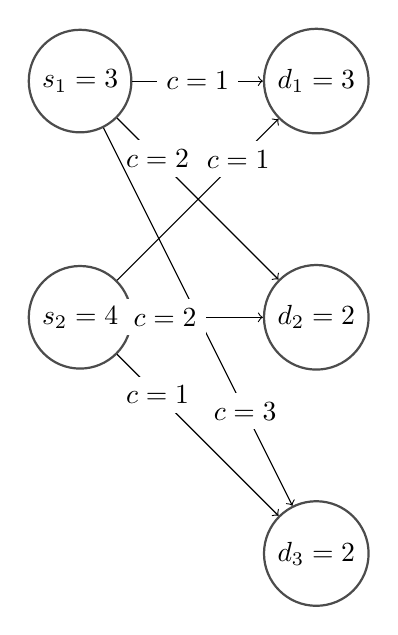
\begin{tikzpicture}[
node/.style={circle, draw=black!70, fill=white!5,  thick, minimum size=9mm}
]
%Nodes
\node[node]      (s1)                                        {$s_1= 3$};
\node[node]      (s2)     [below of =s1, yshift= -2cm]       {$s_2 = 4$};
\node[node]      (d1)     [right of =s1 , xshift= 2cm]       {$d_1 = 3$};
\node[node]      (d2)     [below of = d1, yshift= -2cm]       {$d_2 = 2$};
\node[node]      (d3)     [below of = d2, yshift= -2cm]      {$d_3 = 2$};
%Lines
\draw[->] (s1) -- (d1) node [midway, fill=white] {$c= 1$};
\draw[->] (s1) -- (d2) node [near start, fill=white] {$c = 2$};
\draw[->] (s1) -- (d3) node [near end, fill=white] {$c = 3$};
\draw[->] (s2) -- (d1) node [near end, fill=white] {$c = 1$};
\draw[->] (s2) -- (d2) node [near start, fill=white] {$c = 2$};
\draw[->] (s2) -- (d3) node [near start, fill=white] {$c = 1$};
\end{tikzpicture}
\caption{This picture represents the network for which we will be finding minimum cost flow. The supply and demand nodes are labeled with their corresponding capacities.  The edges between each supply and demand node are labeled according to their cost. To make the problem easier, you can assume all edges have unlimited capacity meaning suppliers can send as much goods as they want over them.}
\label{fig:example1}
\end{framed}
\end{figure}

\begin{figure}[!htb]
\centering
\begin{framed}
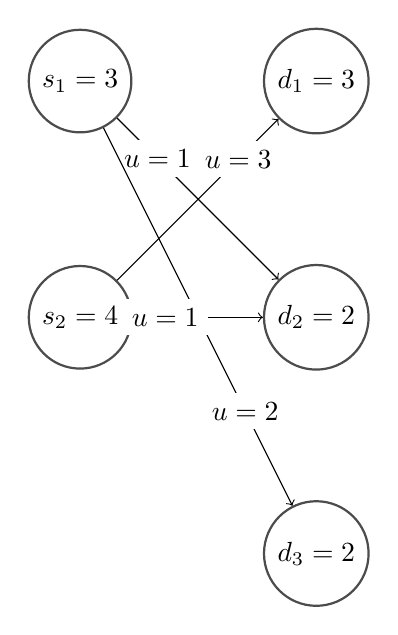
\begin{tikzpicture}[
node/.style={circle, draw=black!70, fill=white!5,  thick, minimum size=9mm}
]
%Nodes
\node[node]      (s1)                                        {$s_1= 3$};
\node[node]      (s2)     [below of =s1, yshift= -2cm]       {$s_2 = 4$};
\node[node]      (d1)     [right of =s1 , xshift= 2cm]       {$d_1 = 3$};
\node[node]      (d2)     [below of = d1, yshift= -2cm]       {$d_2 = 2$};
\node[node]      (d3)     [below of = d2, yshift= -2cm]      {$d_3 = 2$};
%Lines
\draw[->] (s1) -- (d2) node [near start, fill=white] {$u = 1$};
\draw[->] (s1) -- (d3) node [near end, fill=white] {$u = 2$};
\draw[->] (s2) -- (d1) node [near end, fill=white] {$u = 3$};
\draw[->] (s2) -- (d2) node [near start, fill=white] {$u = 1$};
\end{tikzpicture}
\caption{The algorithm starts by matching the capacities on the supply nodes with the capacities on the demand nodes. This is trivial because there are no edge capacities and every node is connected.}
\label{fig:example2}
\end{framed}
\end{figure}

\begin{figure}[!htb]
\centering
\begin{framed}
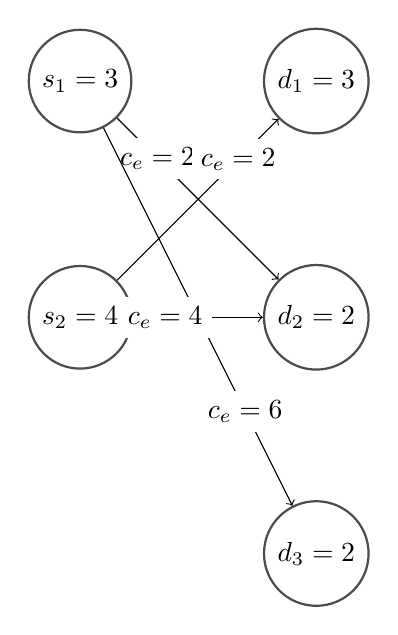
\begin{tikzpicture}[
node/.style={circle, draw=black!70, fill=white!5,  thick, minimum size=9mm}
]
%Nodes
\node[node]      (s1)                                        {$s_1= 3$};
\node[node]      (s2)     [below of =s1, yshift= -2cm]       {$s_2 = 4$};
\node[node]      (d1)     [right of =s1 , xshift= 2cm]       {$d_1 = 3$};
\node[node]      (d2)     [below of = d1, yshift= -2cm]       {$d_2 = 2$};
\node[node]      (d3)     [below of = d2, yshift= -2cm]      {$d_3 = 2$};
%Lines
\draw[->] (s1) -- (d2) node [near start, fill=white] {$c_e = 2$};
\draw[->] (s1) -- (d3) node [near end, fill=white] {$c_e = 6$};
\draw[->] (s2) -- (d1) node [near end, fill=white] {$c_e = 2$};
\draw[->] (s2) -- (d2) node [near start, fill=white] {$c_e = 4$};
\end{tikzpicture}
\caption{This solution is not optimal in terms of cost (yet). I've labled each edge in this figure with the cost each edge has incurred. It works out to 14. The edge costs are just the amount of flow on each edge times its cost.}
\label{fig:example3}
\end{framed}
\end{figure}

\begin{figure}[!htb]
\centering
\begin{framed}
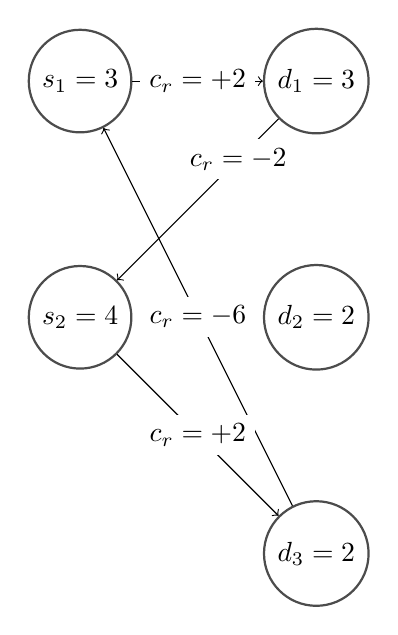
\begin{tikzpicture}[
node/.style={circle, draw=black!70, fill=white!5,  thick, minimum size=9mm}
]
%Nodes
\node[node]      (s1)                                        {$s_1= 3$};
\node[node]      (s2)     [below of =s1, yshift= -2cm]       {$s_2 = 4$};
\node[node]      (d1)     [right of =s1 , xshift= 2cm]       {$d_1 = 3$};
\node[node]      (d2)     [below of = d1, yshift= -2cm]       {$d_2 = 2$};
\node[node]      (d3)     [below of = d2, yshift= -2cm]      {$d_3 = 2$};
%Lines
\draw[->] (s1) -- (d1) node [midway, fill=white] {$c_r=+2$};
\draw[<-] (s1) -- (d3) node [midway, fill=white] {$c_r= -6$};
\draw[<-] (s2) -- (d1) node [near end, fill=white] {$c_r=-2 $};
\draw[->] (s2) -- (d3) node [midway, fill=white] {$c_r=+2$};
\end{tikzpicture}
\caption{In order to improve the cost of flow through the network, we look for a reduced cost cycle. The cycle needs to start and end on the same node. It also needs to alternate between suppliers and demand nodes. This is because you delete costly edges and replace them with less expensive ones. By traversing the cycle we see can reduce the cost by 4 to the optimal amount. Edges in the cycle are labeled with their reduced cost (i.e. how much they improve the total cost)}
\label{fig:example4}
\end{framed}
\end{figure}

\begin{figure}[!htb]
\centering
\begin{framed}
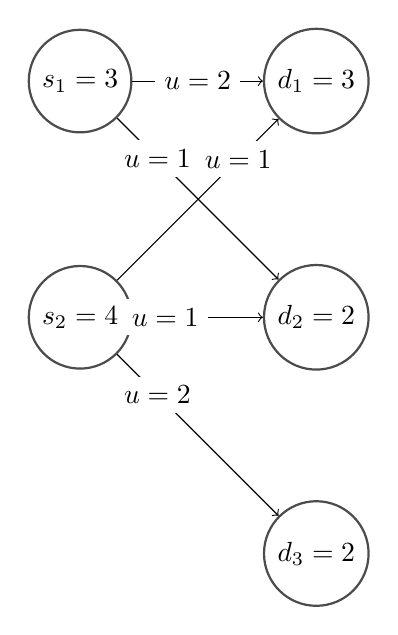
\begin{tikzpicture}[
node/.style={circle, draw=black!70, fill=white!5,  thick, minimum size=9mm}
]
%Nodes
\node[node]      (s1)                                        {$s_1= 3$};
\node[node]      (s2)     [below of =s1, yshift= -2cm]       {$s_2 = 4$};
\node[node]      (d1)     [right of =s1 , xshift= 2cm]       {$d_1 = 3$};
\node[node]      (d2)     [below of = d1, yshift= -2cm]       {$d_2 = 2$};
\node[node]      (d3)     [below of = d2, yshift= -2cm]      {$d_3 = 2$};
%Lines
\draw[->] (s1) -- (d1) node [midway, fill=white] {$u=2$};
\draw[->] (s1) -- (d2) node [near start, fill=white] {$u=1$};
\draw[->] (s2) -- (d1) node [near end, fill=white] {$u=1$};
\draw[->] (s2) -- (d2) node [near start, fill=white] {$u=1$};
\draw[->] (s2) -- (d3) node [near start, fill=white] {$u=2$};
\end{tikzpicture}
\caption{At this point, there are no more reduced cost cycles, so we've found an optimal solution in terms of cost. The edges reflect the amount of units flowing from supply to demand in this solution.}
\label{fig:example5}
\end{framed}
\end{figure}

\begin{figure}[!htb]
\centering
\begin{framed}
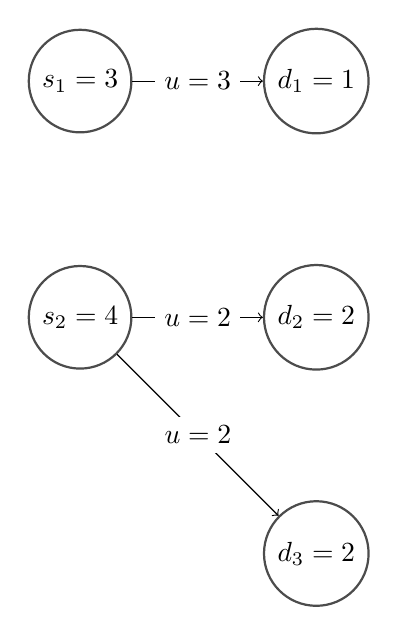
\begin{tikzpicture}[
node/.style={circle, draw=black!70, fill=white!5,  thick, minimum size=9mm}
]
%Nodes
\node[node]      (s1)                                        {$s_1= 3$};
\node[node]      (s2)     [below of =s1, yshift= -2cm]       {$s_2 = 4$};
\node[node]      (d1)     [right of =s1 , xshift= 2cm]       {$d_1 = 1$};
\node[node]      (d2)     [below of = d1, yshift= -2cm]       {$d_2 = 2$};
\node[node]      (d3)     [below of = d2, yshift= -2cm]      {$d_3 = 2$};
%Lines
\draw[->] (s1) -- (d1) node [midway, fill=white] {$u=3$};
\draw[->] (s2) -- (d2) node [midway, fill=white] {$u=2$};
\draw[->] (s2) -- (d3) node [midway, fill=white] {$u=2$};
\end{tikzpicture}
\caption{As long as there aren't minimum cost cycles we've found a solution. Zero-cost cycles exists in this simple network. As a result, there is more than 1 solution that optimizes cost and flow. This figure shows that example.}
\label{fig:example6}
\end{framed}
\end{figure}

\begin{figure}[!htb]
\centering
\begin{framed}
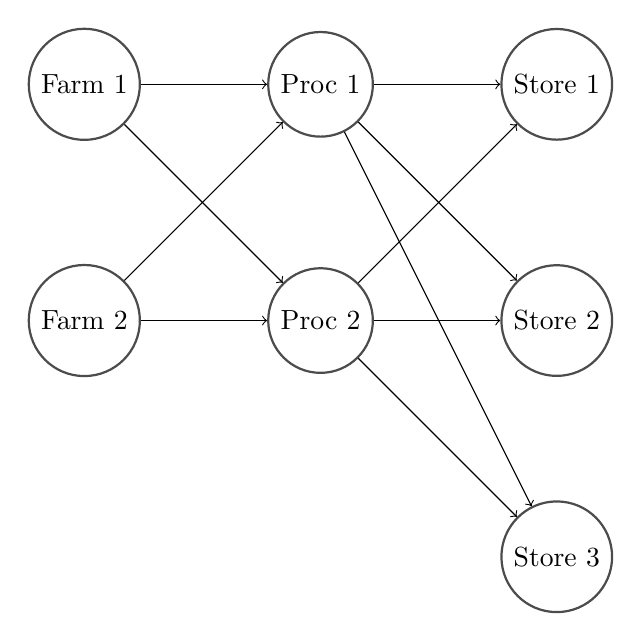
\begin{tikzpicture}[
node/.style={circle, draw=black!70, fill=white!5,  thick, minimum size=9mm}
]
%Nodes
\node[node]      (f1)                                        {Farm 1};
\node[node]      (f2)     [below of = f1, yshift= -2cm]       {Farm 2};
\node[node]      (p1)    [right of = f1, xshift= 2cm]        {Proc 1};
\node[node]      (p2)     [below of =p1, yshift= -2cm]       {Proc 2};
\node[node]      (s1)     [right of = p1 , xshift= 2cm]       {Store 1};
\node[node]      (s2)     [below of = s1, yshift= -2cm]       {Store 2};
\node[node]      (s3)     [below of = s2, yshift= -2cm]      {Store 3};
%Lines
\draw[->] (f1) -- (p1) ;%node [midway, fill=white] {};
\draw[->] (f1) -- (p2) ;%node [near start, fill=white] {};
\draw[->] (f2) -- (p1) ;%node [near start, fill=white] {distance};
\draw[->] (f2) -- (p2) ;%node [midway, fill=white] {distance};
\draw[->] (p1) -- (s1) ;%node [midway, fill=white] {distance};
\draw[->] (p1) -- (s2) ;%node [near start, fill=white] {distance};
\draw[->] (p1) -- (s3) ;%node [near end, fill=white] {distance};
\draw[->] (p2) -- (s1) ;%node [near end, fill=white] {distance};
\draw[->] (p2) -- (s2) ;%node [midway, fill=white] {distance};
\draw[->] (p2) -- (s3) ;%node [near start, fill=white] {distance};
\end{tikzpicture}
\caption{This figure show the structure of the agricultural supply network in my model. Farms grow crops and send their product to intermediate processors. Processors send their product to stores. The processors and farms send their product to the next step in the network using local roads. They choose where to send their crops based on convenience.}
\label{fig:spec}
\end{framed}
\end{figure}

\section{Maps}

\begin{sidewaysfigure}[!htb]
\centering
\begin{framed}
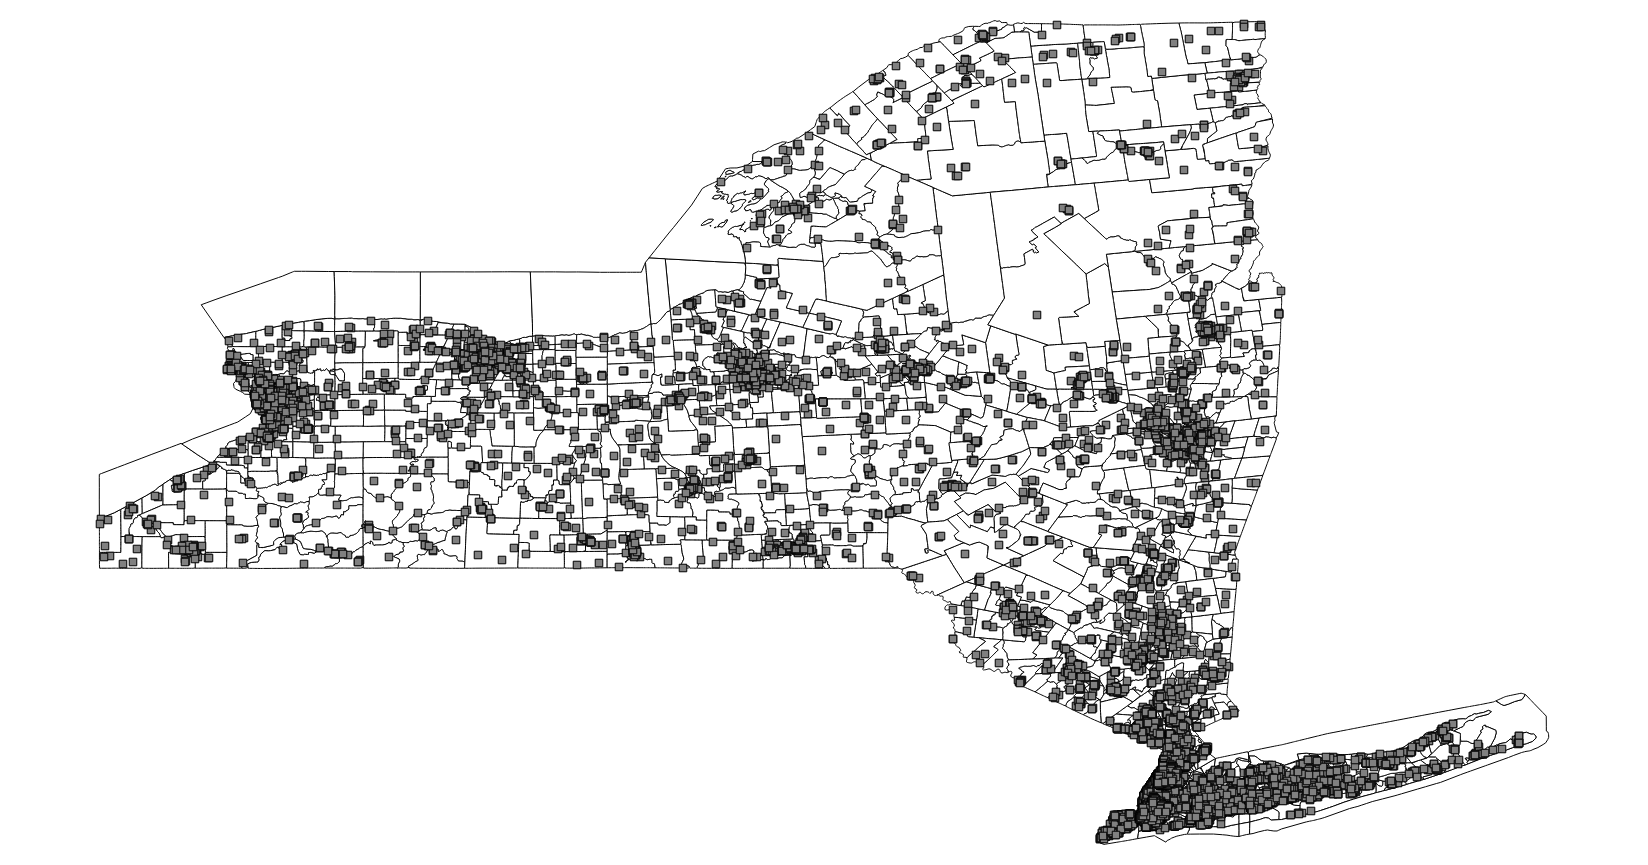
\includegraphics[scale=.50]{map_3}
\caption{Here I've mapped all the stores as grey squares. They've been over-layed on top of the census tracts so you can see that stores are spread out between them. You can see are much more sparsely spread in the center of the state.}
\label{fig:map_3}
\end{framed}
\end{sidewaysfigure}

\begin{sidewaysfigure}[!htb]
\centering
\begin{framed}
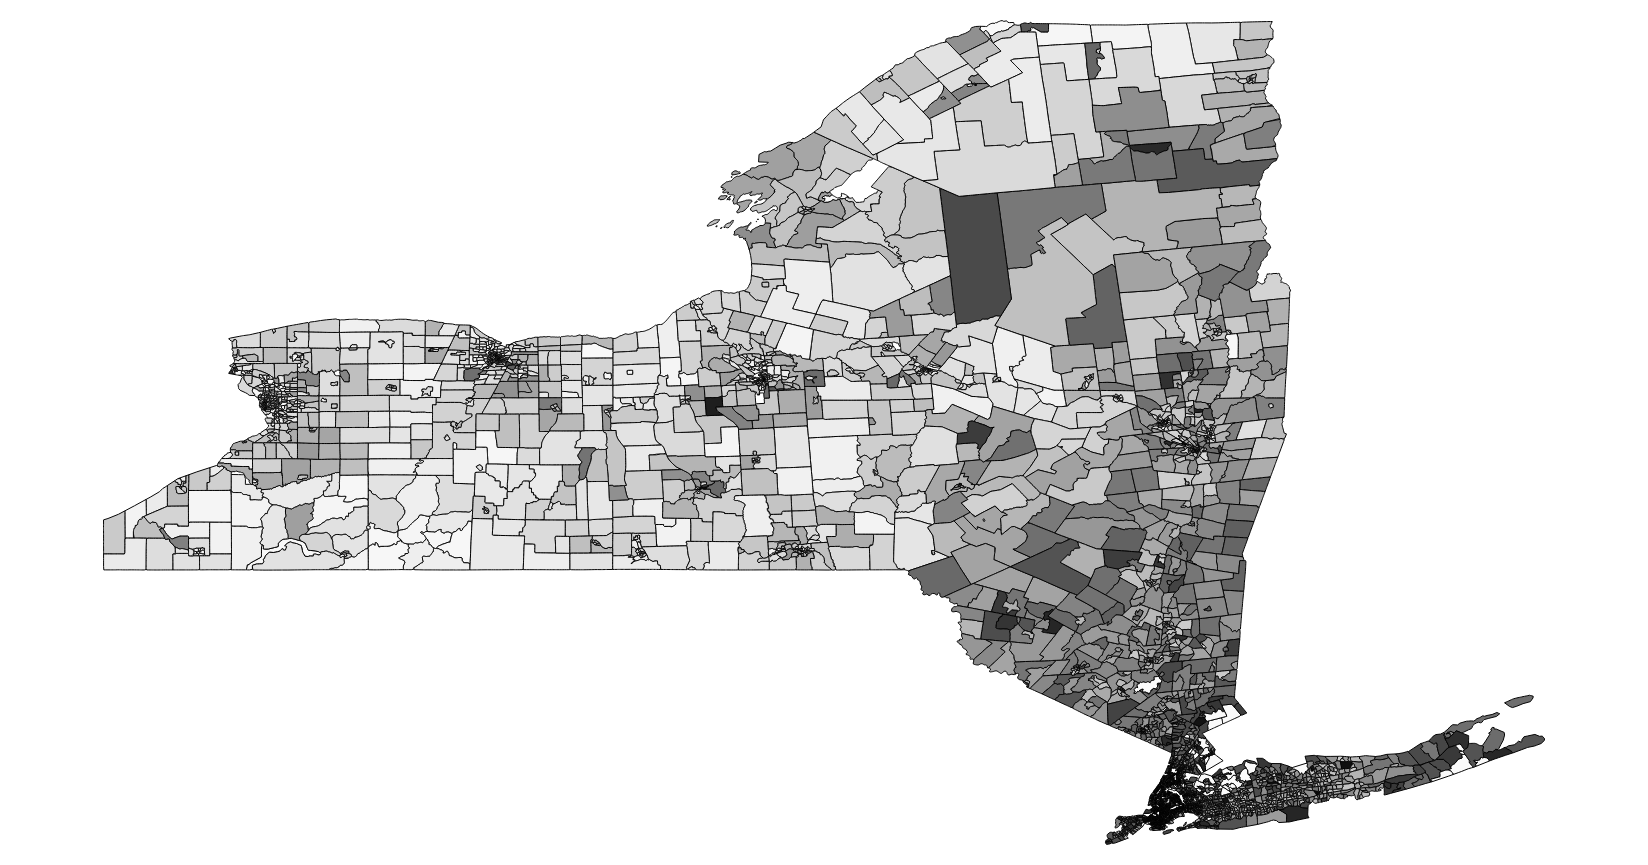
\includegraphics[scale=.50]{map_4}
\caption{The purpose of this map shows the distribution of median housing values through out the census tracts. The darker the shading, the higher the median property value for that tract. You can see housing is relatively cheap in western and northern New York, but expensive in the south western corner of the state.}
\label{fig:map_4}
\end{framed}
\end{sidewaysfigure}

%%%%%%%%%%%%%%%%%%%%%%%%%%%%%%%%%%%%%%%%%%%%%%%%%%%%%%%%%%%%%%%%%
%Farms%%%%%%%%%%%%%%%%%%%%%%%%%%%%%%%%%%%%%%%%%%%%%%%%%%%%%%%%%%%
%%%%%%%%%%%%%%%%%%%%%%%%%%%%%%%%%%%%%%%%%%%%%%%%%%%%%%%%%%%%%%%%%

\begin{sidewaysfigure}[!htb]
\centering
\begin{framed}
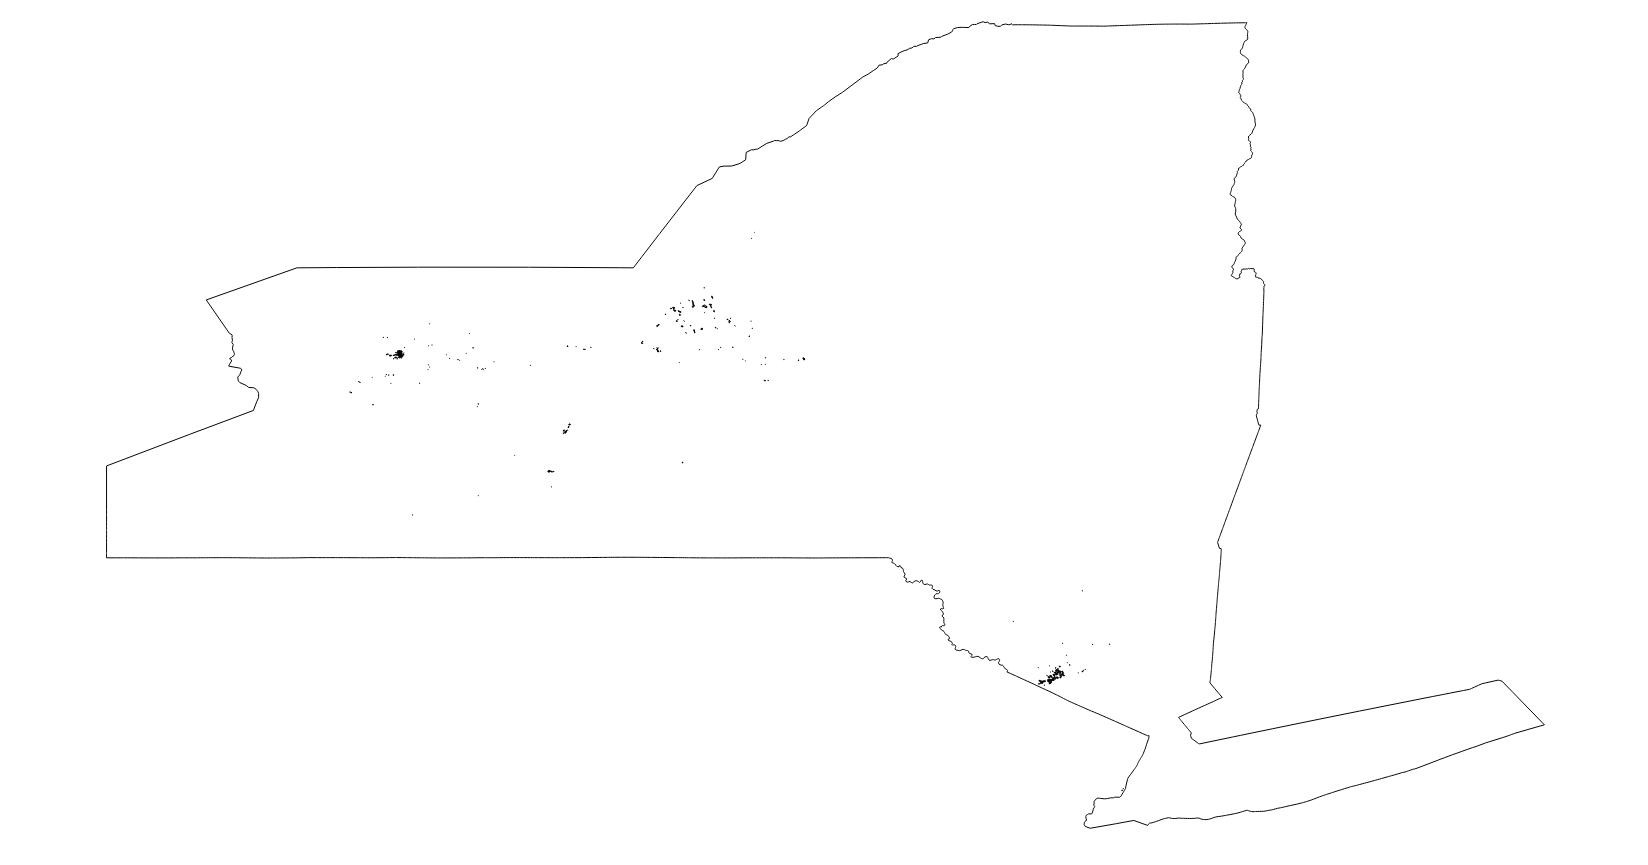
\includegraphics[scale=.50]{farms_49}
\caption{This figure shows the location of onion farms based on the cropland data put through the sieve. If you are interested in descriptive statistics of the farms you can see Table \ref{tab:farms}. You can see there are roughly four clusters of farms. Three of them are in the center of the state, and the fourth is south. The locations of farms influenced the prices.}
\label{fig:farms_49}
\end{framed}
\end{sidewaysfigure}

\begin{sidewaysfigure}[!htb]
\centering
\begin{framed}
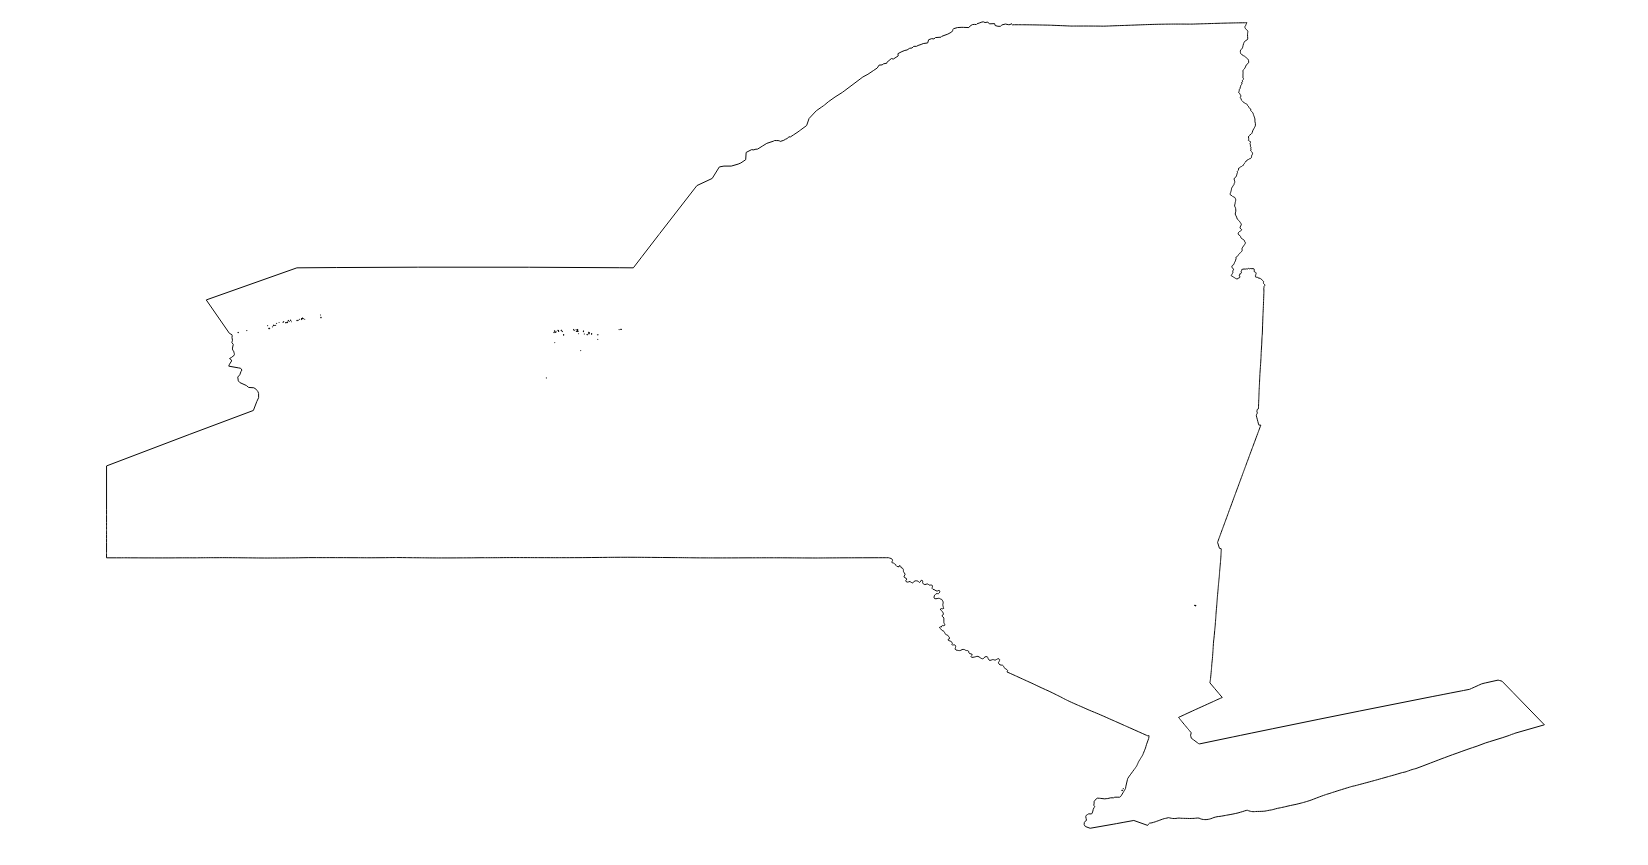
\includegraphics[scale=.50]{farms_66}
\caption{This figure shows the location of cherry farms based on the cropland data put through the sieve. Cherries had the least amount of area dedicated to them and the farms were scattered throughout the far west portion of the state. As a result, the prices in the cherry band are relatively higher. If you are interested in descriptive statistics of the farms you can see Table \ref{tab:farms}.}
\label{fig:farms_66}
\end{framed}
\end{sidewaysfigure}

\begin{sidewaysfigure}[!htb]
\centering
\begin{framed}
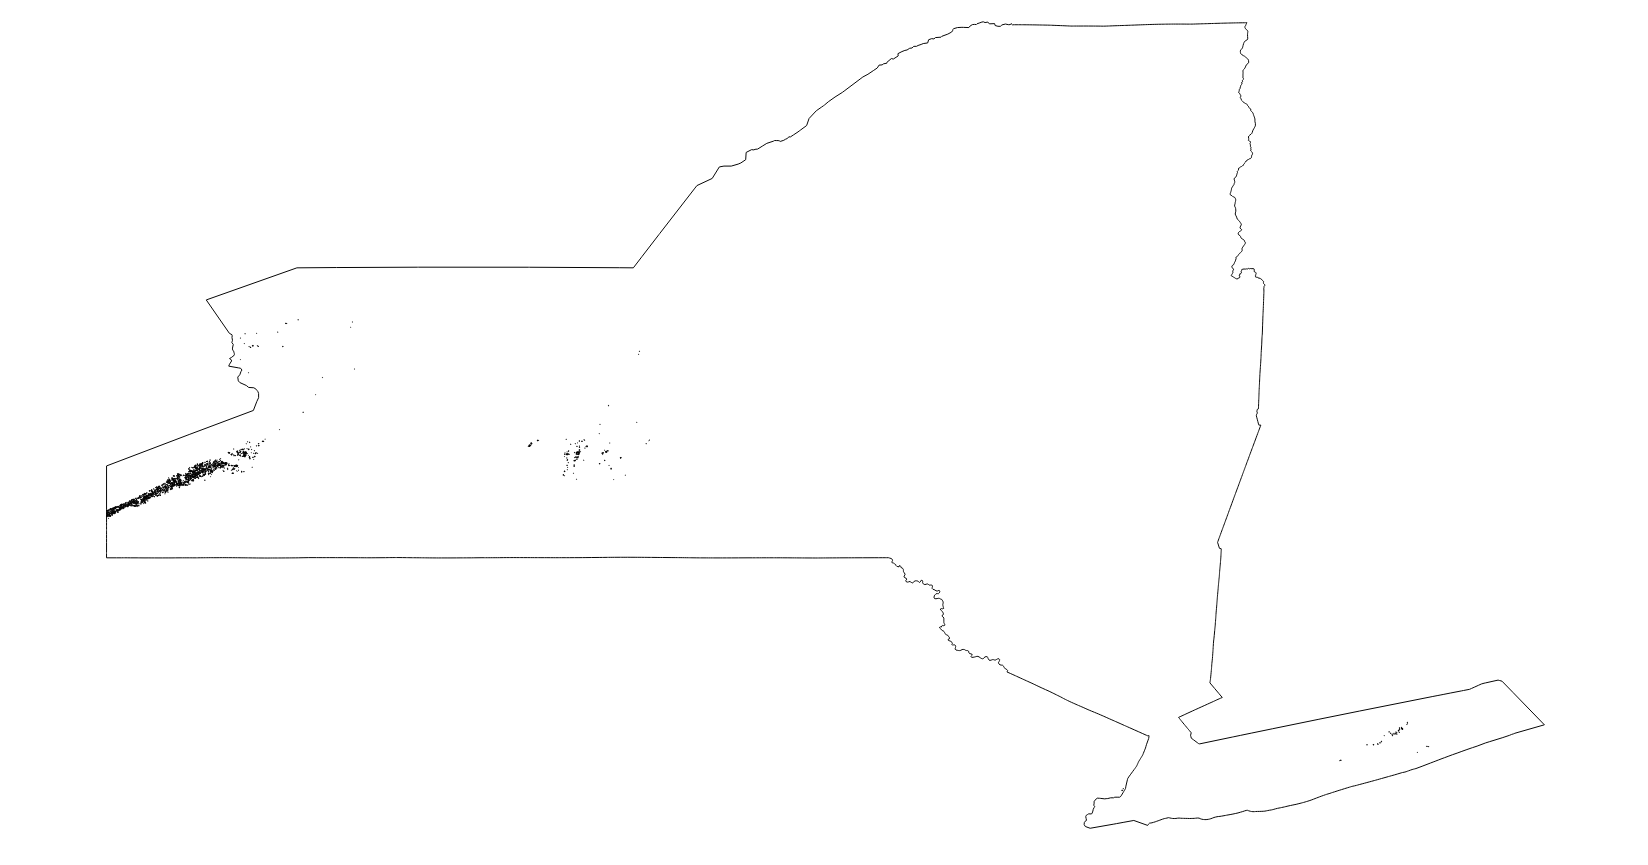
\includegraphics[scale=.50]{farms_69}
\caption{This figure shows the location of grape farms based on the cropland data put through the sieve. There is a dense band of farms in the south west portion of the state. There are smaller clusters in the south central part of the state and the northwest. If you are interested in descriptive statistics of the farms you can see Table \ref{tab:farms}.}
\label{fig:farms_69}
\end{framed}
\end{sidewaysfigure}

\begin{sidewaysfigure}[!htb]
\centering
\begin{framed}
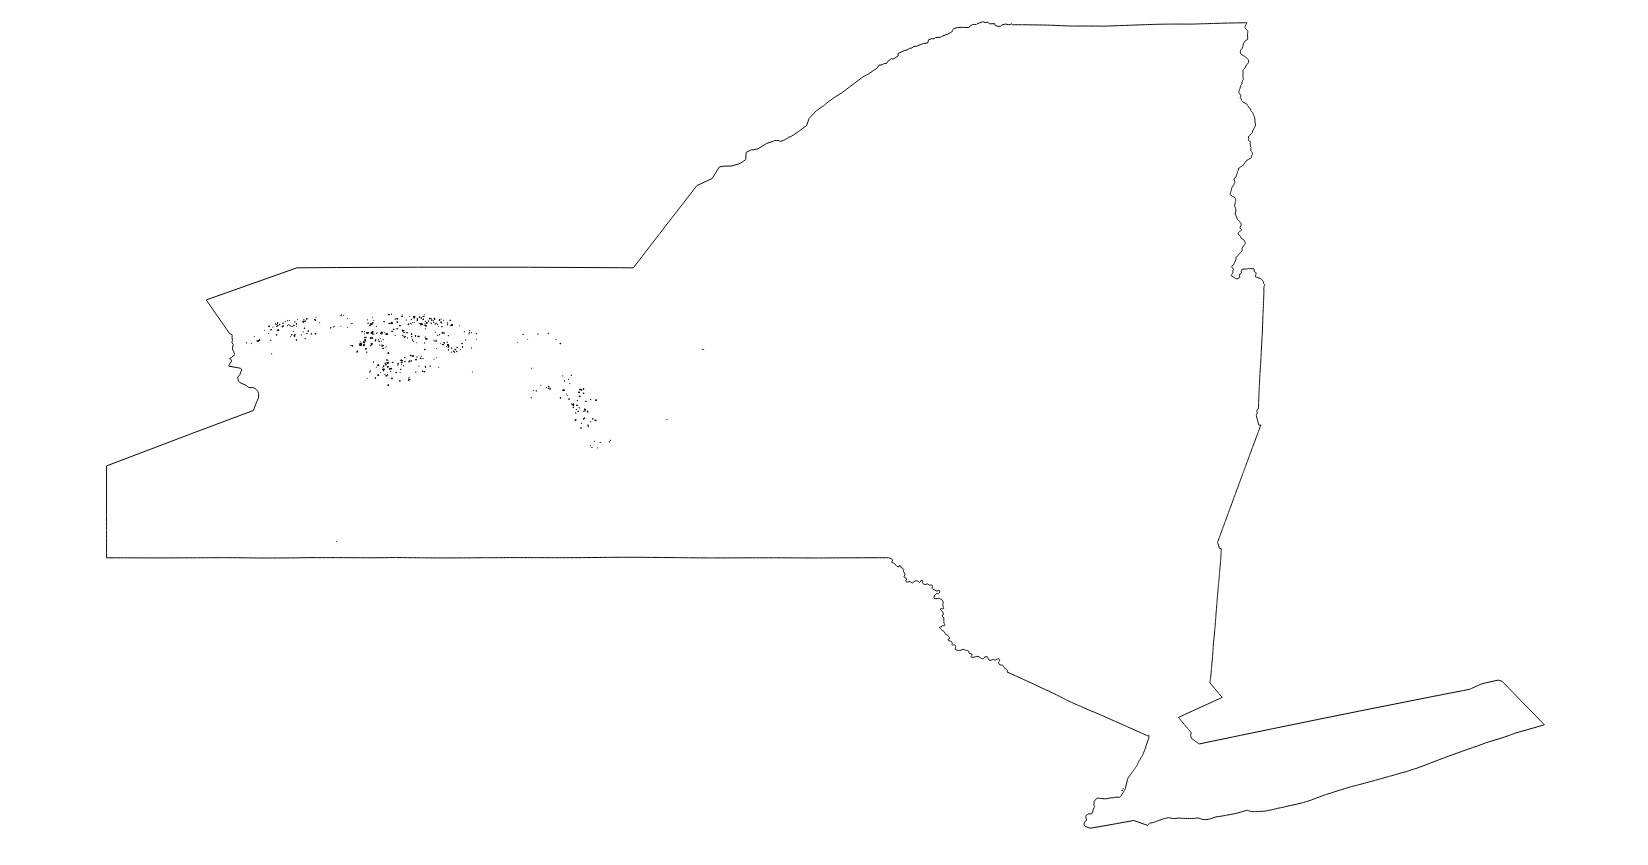
\includegraphics[scale=.50]{farms_243}
\caption{This figure shows the location of cabbage farms based on the cropland data put through the sieve. The cabbage farms are relatively spread out compared to the other bands. If you are interested in descriptive statistics of the farms you can see Table \ref{tab:farms}.}
\label{fig:farms_243}
\end{framed}
\end{sidewaysfigure}

%%%%%%%%%%%%%%%%%%%%%%%%%%%%%%%%%%%%%%%%%%%%%%%%%%%%%%%%%%%%%%%%%
%Network%%%%%%%%%%%%%%%%%%%%%%%%%%%%%%%%%%%%%%%%%%%%%%%%%%%%%%%%%
%%%%%%%%%%%%%%%%%%%%%%%%%%%%%%%%%%%%%%%%%%%%%%%%%%%%%%%%%%%%%%%%%

\begin{sidewaysfigure}[!htb]
\centering
\begin{framed}
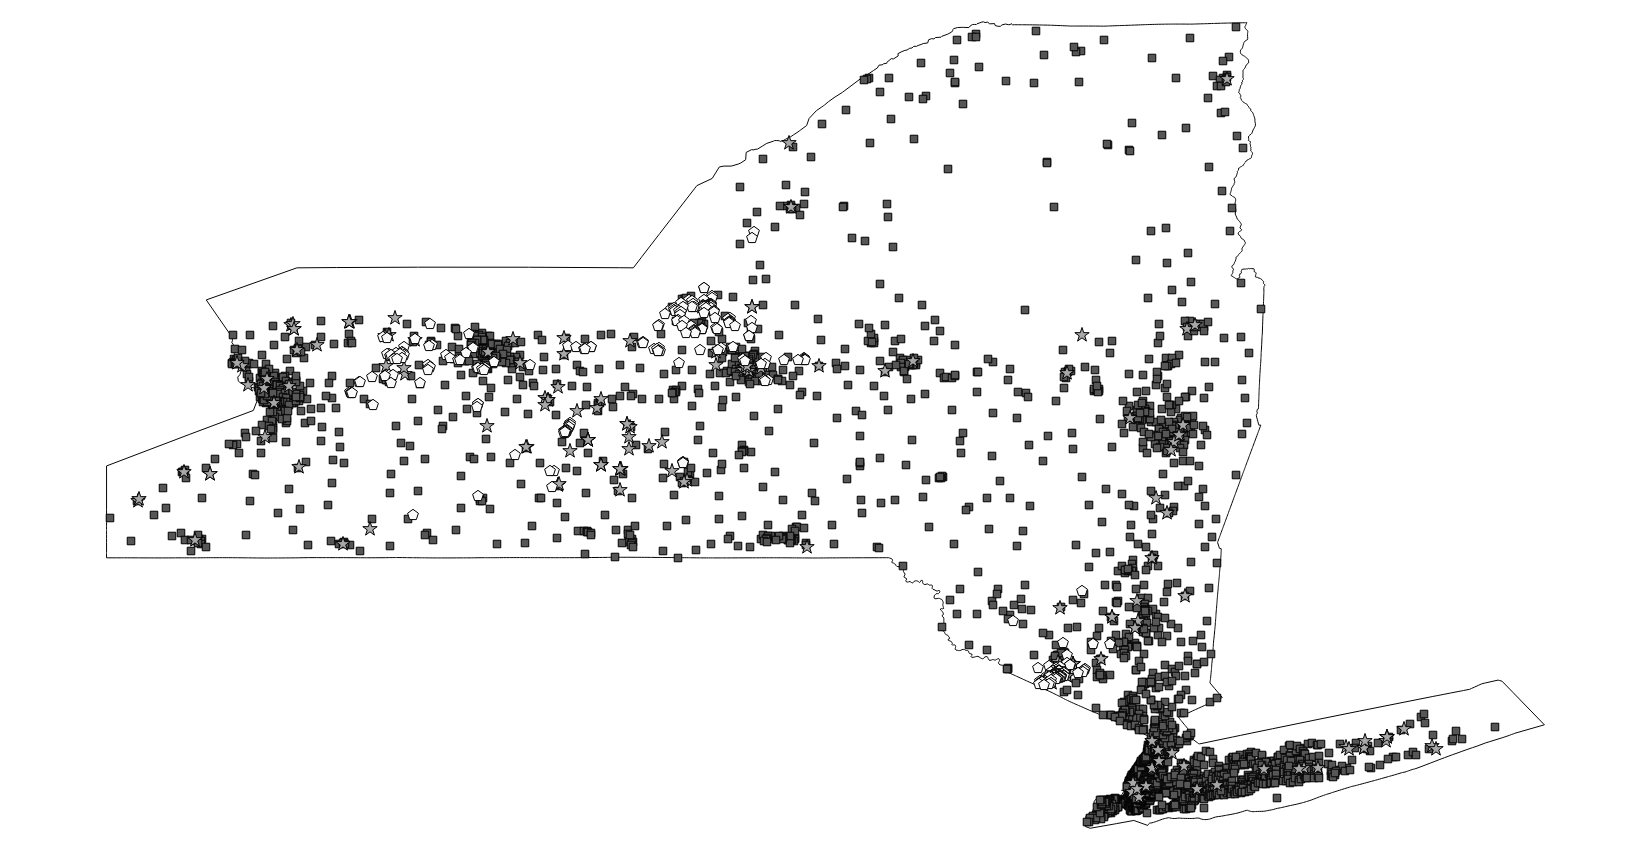
\includegraphics[scale=.50]{network_49}
\caption{This figure visualizes onion supply network in New York. The pentagons are farms, the stars are processors, and the squares are stores. Onions had the second highest number of intermediate dealers to choose from as you can see in Table \ref{tab:procs}}
\label{fig:network_49}
\end{framed}
\end{sidewaysfigure}

\begin{sidewaysfigure}[!htb]
\centering
\begin{framed}
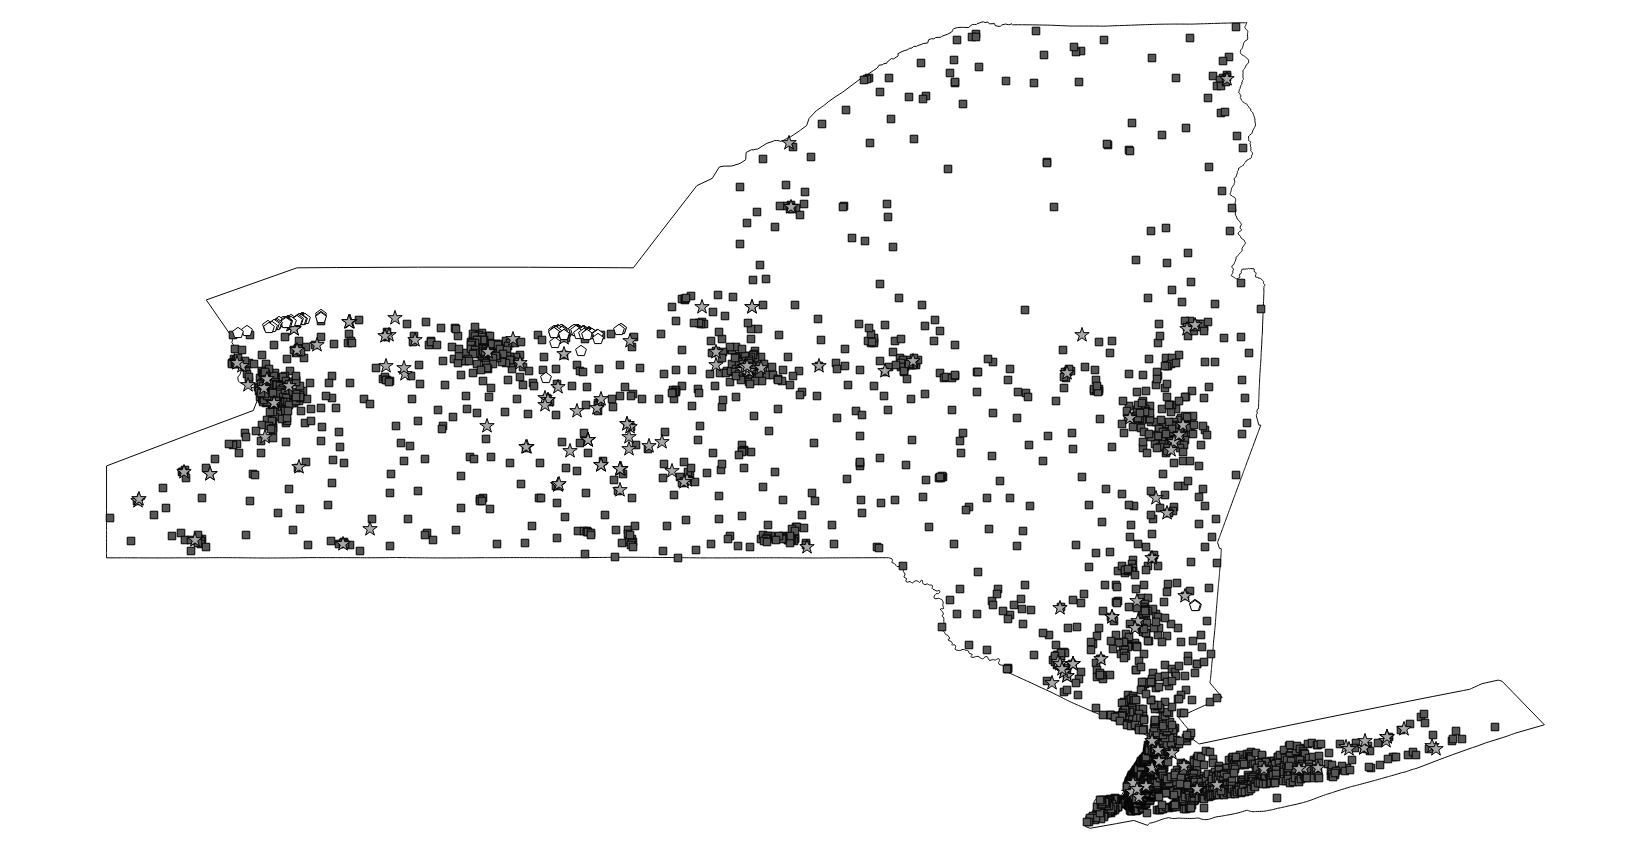
\includegraphics[scale=.50]{network_66}
\caption{This figure tries to visualize the cherries supply network in New York. The pentagons are farms, the stars are processors, and the squares are stores. You can see how many dealers there were in the other table. The cherries had the least amount of dealers dedicated to them so prices are highest at the cherries. }
\label{fig:network_66}
\end{framed}
\end{sidewaysfigure}

\begin{sidewaysfigure}[!htb]
\centering
\begin{framed}
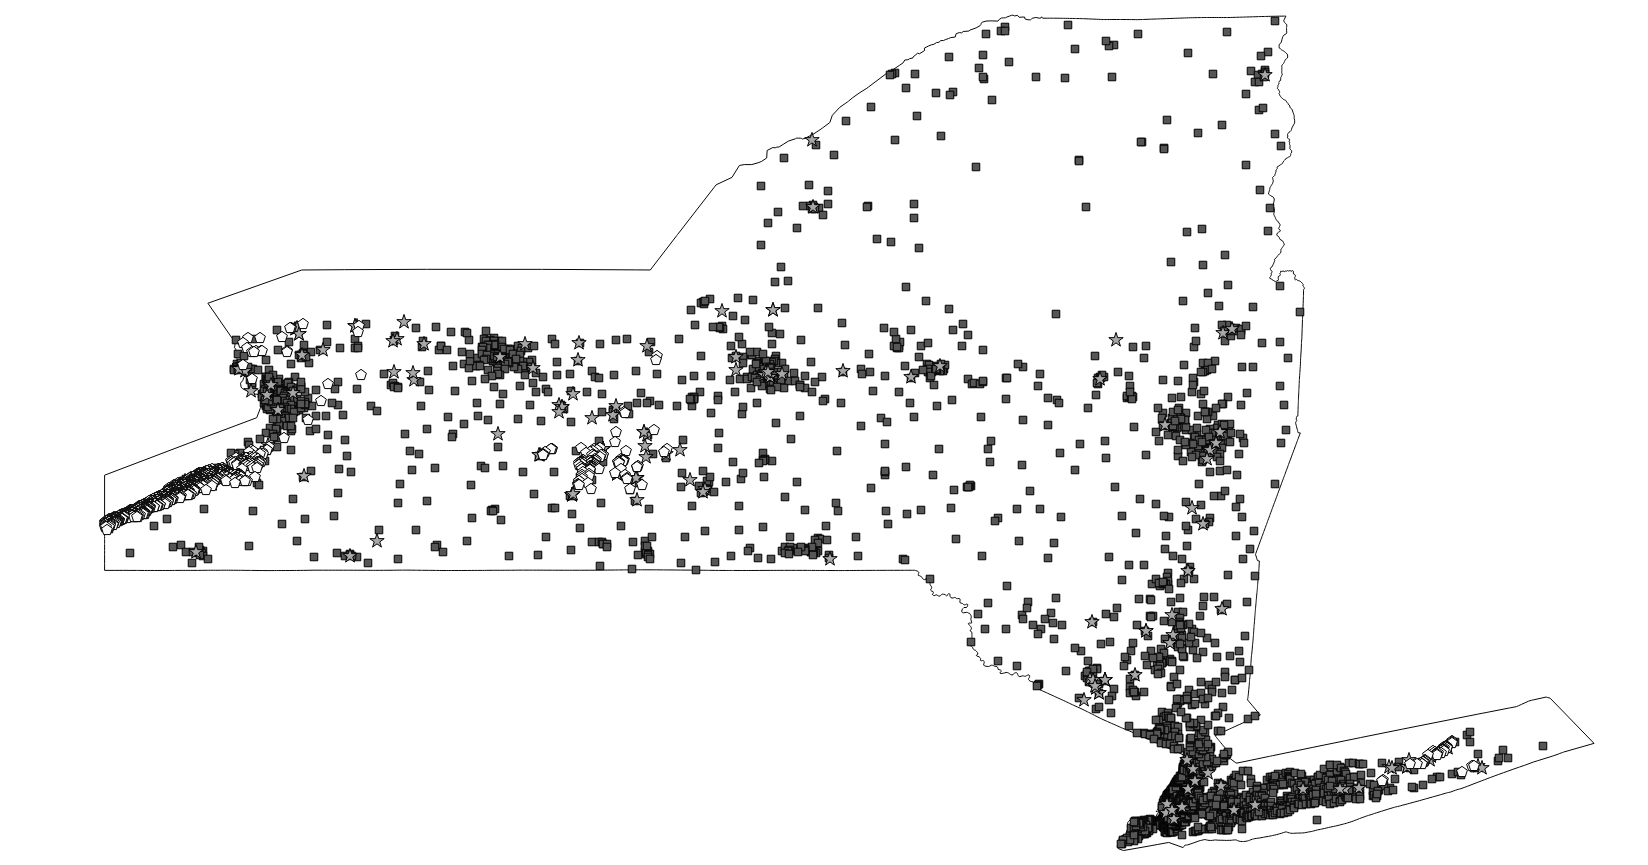
\includegraphics[scale=.50]{network_69}
\caption{This figure tries to visualize the grape supply network in New York. The pentagons are farms, the stars are processors, and the squares are stores. You can see how many dealers there were in Table \ref{tab:procs}. }
\label{fig:network_69}
\end{framed}
\end{sidewaysfigure}

\begin{sidewaysfigure}[!htb]
\centering
\begin{framed}
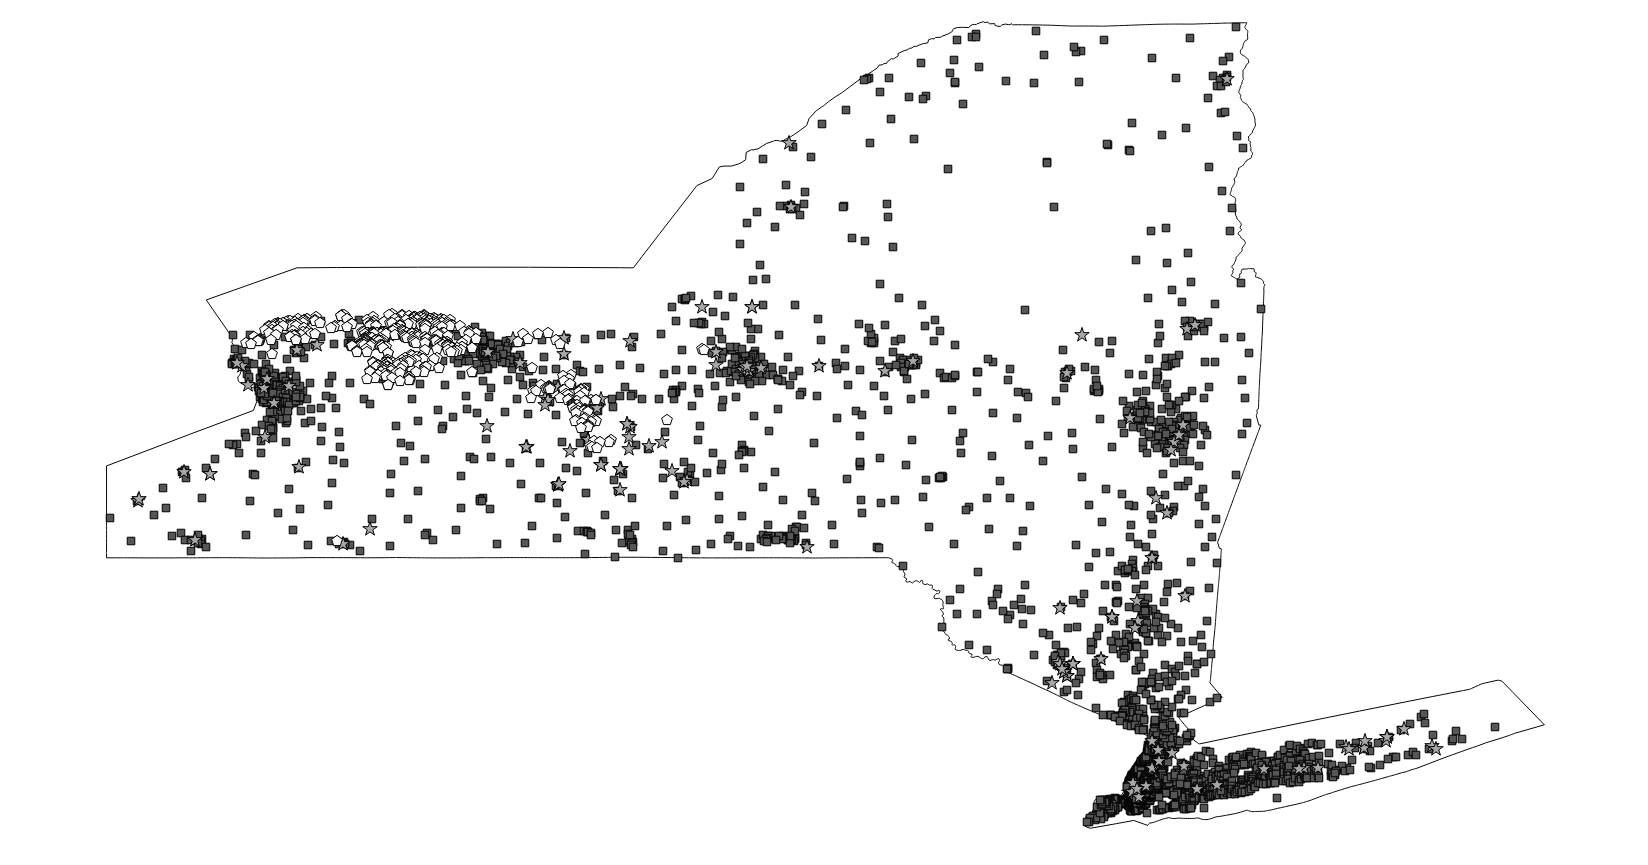
\includegraphics[scale=.50]{network_243}
\caption{This figure tries to visualize the cabbage supply network in New York. The pentagons are farms, the stars are processors, and the squares are stores. You can see how many dealers there were in Table \ref{tab:procs}}
\label{fig:network_243}
\end{framed}
\end{sidewaysfigure}

%%%%%%%%%%%%%%%%%%%%%%%%%%%%%%%%%%%%%%%%%%%%%%%%%%%%%%%%%%%%%%%%%
%Prices%%%%%%%%%%%%%%%%%%%%%%%%%%%%%%%%%%%%%%%%%%%%%%%%%%%%%%%%%%
%%%%%%%%%%%%%%%%%%%%%%%%%%%%%%%%%%%%%%%%%%%%%%%%%%%%%%%%%%%%%%%%%

\begin{sidewaysfigure}[!htb]
\centering
\begin{framed}
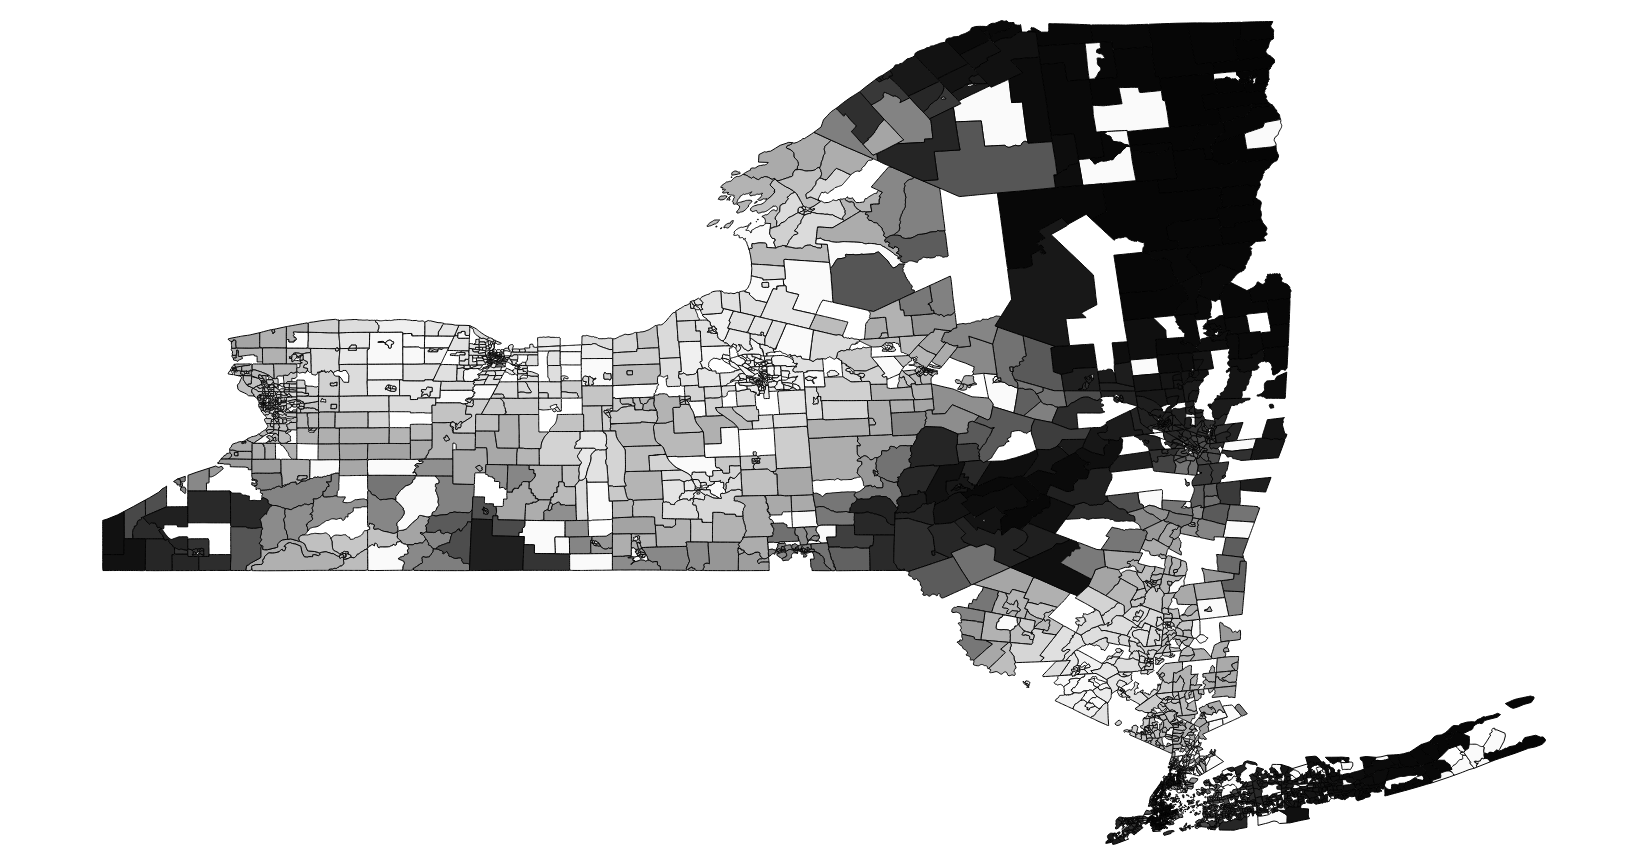
\includegraphics[scale=.50]{prices_49}
\caption{This figure shows the distribution of onion prices through out the state according to the linear program. You can see that the prices are highest in the northeast and southeast corners of the state. The fact that there was a cluster of farms in the southern part of the state caused prices to be lower there compared to some of the other bands.}
\label{fig:prices_49}
\end{framed}
\end{sidewaysfigure}


\begin{sidewaysfigure}[!htb]
\centering
\begin{framed}
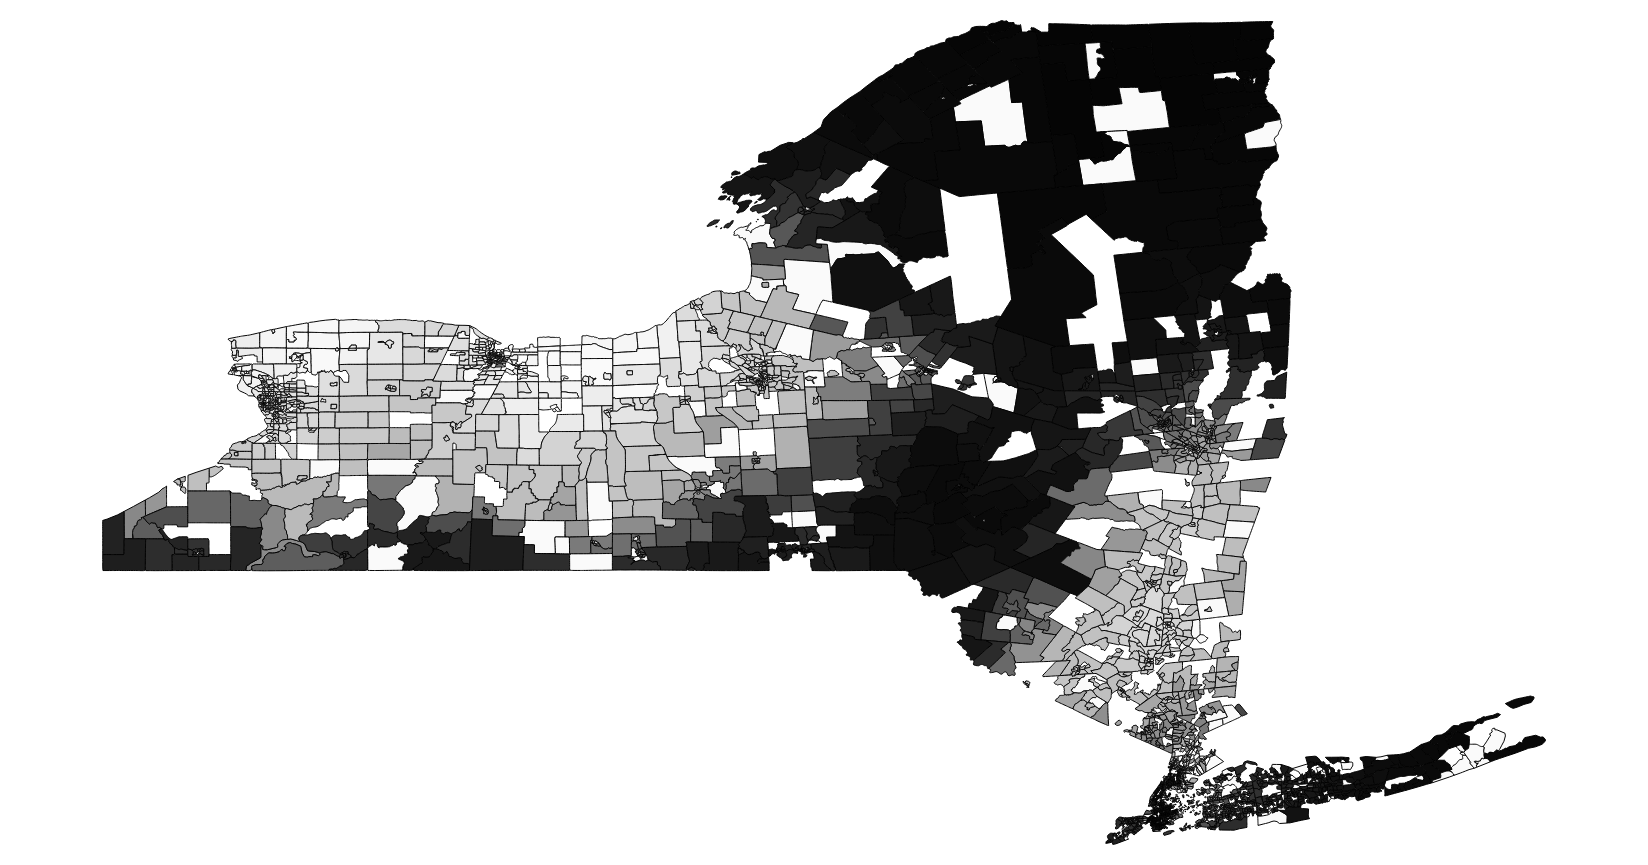
\includegraphics[scale=.50]{prices_66}
\caption{This figure shows the distribution of cherry prices through out the state according to the linear program. The darker the shading the higher the price. You can see that the prices are highest in the northeast and the southeast corners of the states. This reflects these regions relative distance from farms. Prices are high in the northern part of the state because this region focuses on other types of farming, mainly dairy. Prices are high in the south east because land in these areas is not used for farming. }
\label{fig:prices_66}
\end{framed}
\end{sidewaysfigure}


\begin{sidewaysfigure}[!htb]
\centering
\begin{framed}
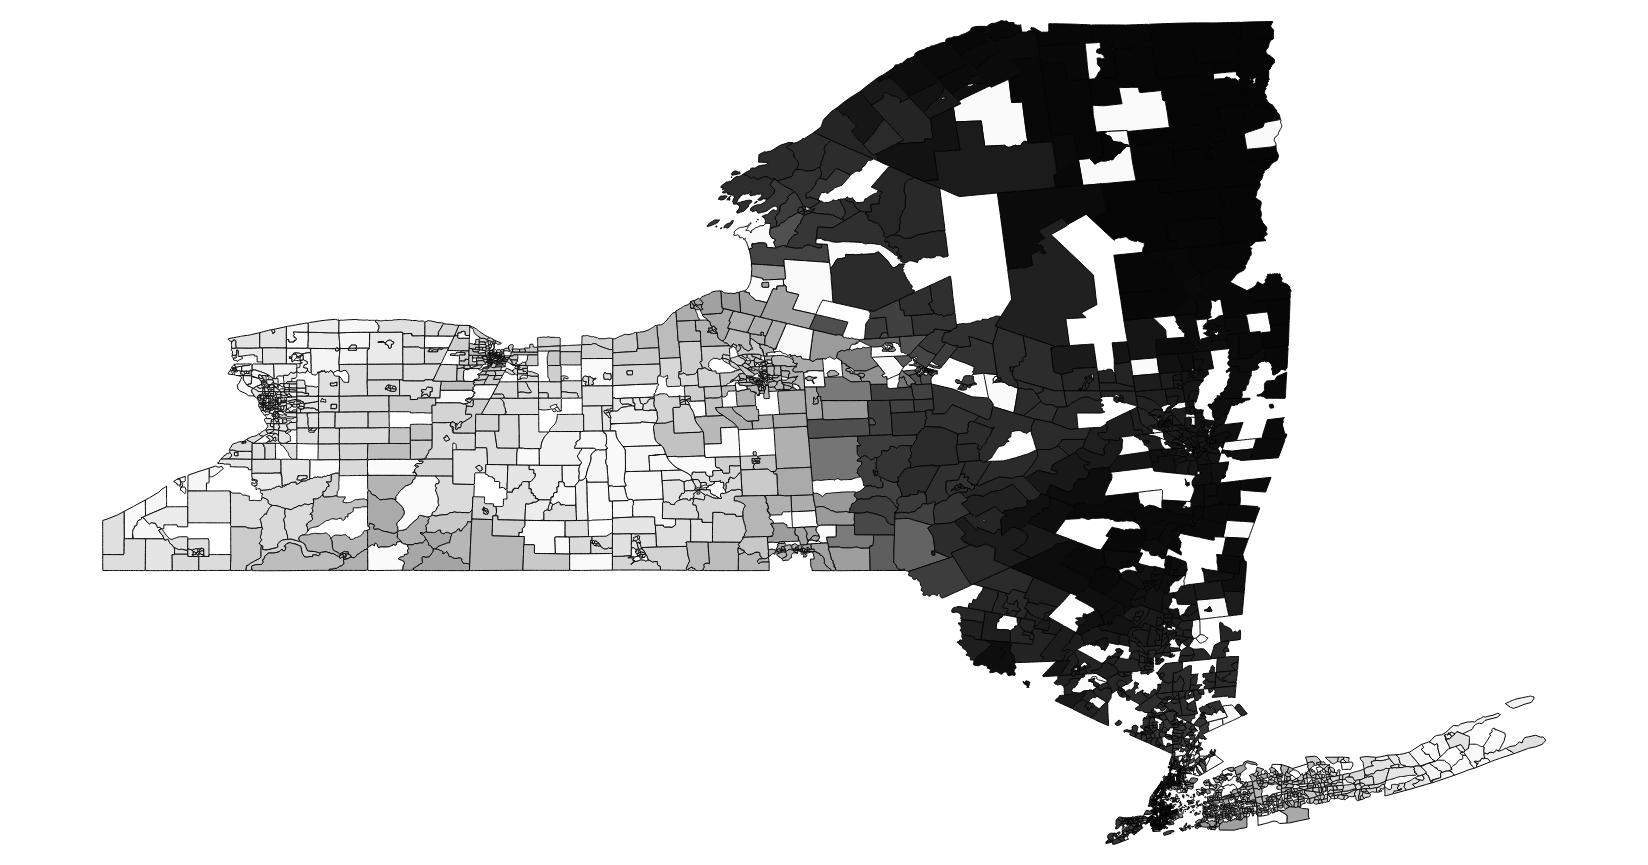
\includegraphics[scale=.50]{prices_69}
\caption{This figure shows the distribution of grape prices through out the state according to the linear program. The darker the shading the higher the price. Because of the farms dense concentration on the western portion of the state, the prices in the west are consistently low when compared to the east. This means you would expect it to be less expensive to find grapes in the western portion of the state because transportation costs are lower.}
\label{fig:prices_69}
\end{framed}
\end{sidewaysfigure}


\begin{sidewaysfigure}[!htb]
\centering
\begin{framed}
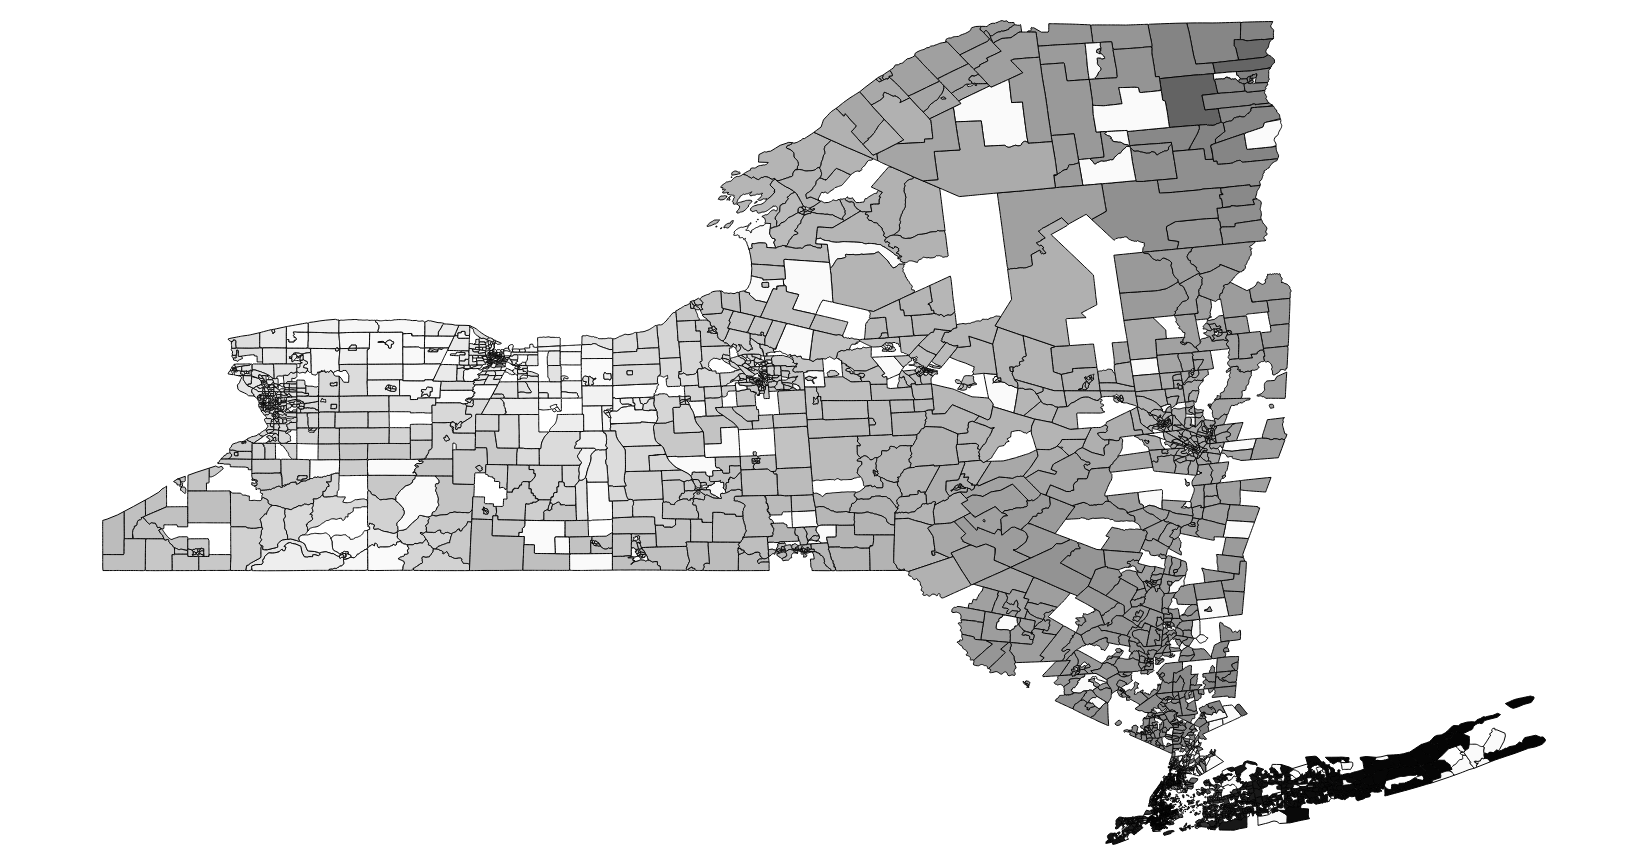
\includegraphics[scale=.50]{prices_243}
\caption{This figure shows the distribution of cabbage prices through out the state according to the linear program. The darker the shading the higher the price. The result for cabbages seems more spread out across the state because of the shading grade. In actuality, the result was similar to the others. However, prices in the southeast are significantly higher for cabbages than the other bands. This variance causes the figure to look more evenly distributed than the other farms. The high prices in the south east reflect the locations of farms.}
\label{fig:prices_243}
\end{framed}
\end{sidewaysfigure}


%%%%%%%%%%%%%%%%%%%%%%%%%%%%%%%%%%%%%%%%%%%%%%%%%%%%%%%%%%%%%%%%%
%price Differences%%%%%%%%%%%%%%%%%%%%%%%%%%%%%%%%%%%%%%%%%%%%%%%
%%%%%%%%%%%%%%%%%%%%%%%%%%%%%%%%%%%%%%%%%%%%%%%%%%%%%%%%%%%%%%%%%

\begin{sidewaysfigure}[!htb]
\centering
\begin{framed}
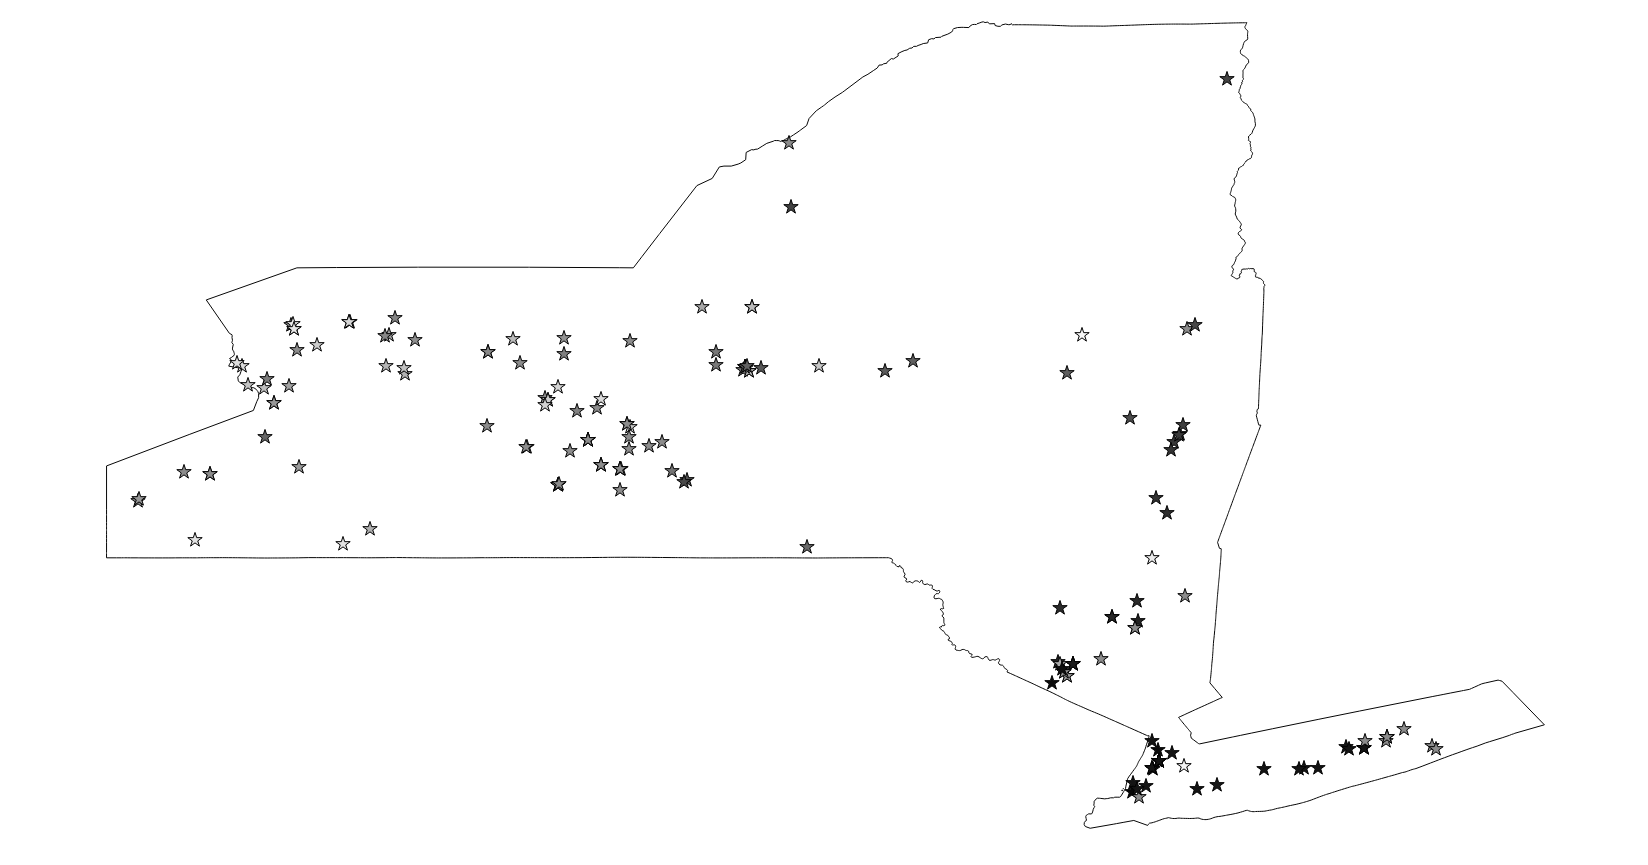
\includegraphics[scale=.50]{procs_243_49}
\caption{This figure compares the difference in prices between onions and cabbages at the intermediaries. I chose cabbages because the result of the linear program was most different for this band. The stars represent the dealers. Darker means onion prices were greater. Lighter means cabbage prices were greater.}
\label{fig:procs_243_49}
\end{framed}
\end{sidewaysfigure}

\begin{sidewaysfigure}[!htb]
\centering
\begin{framed}
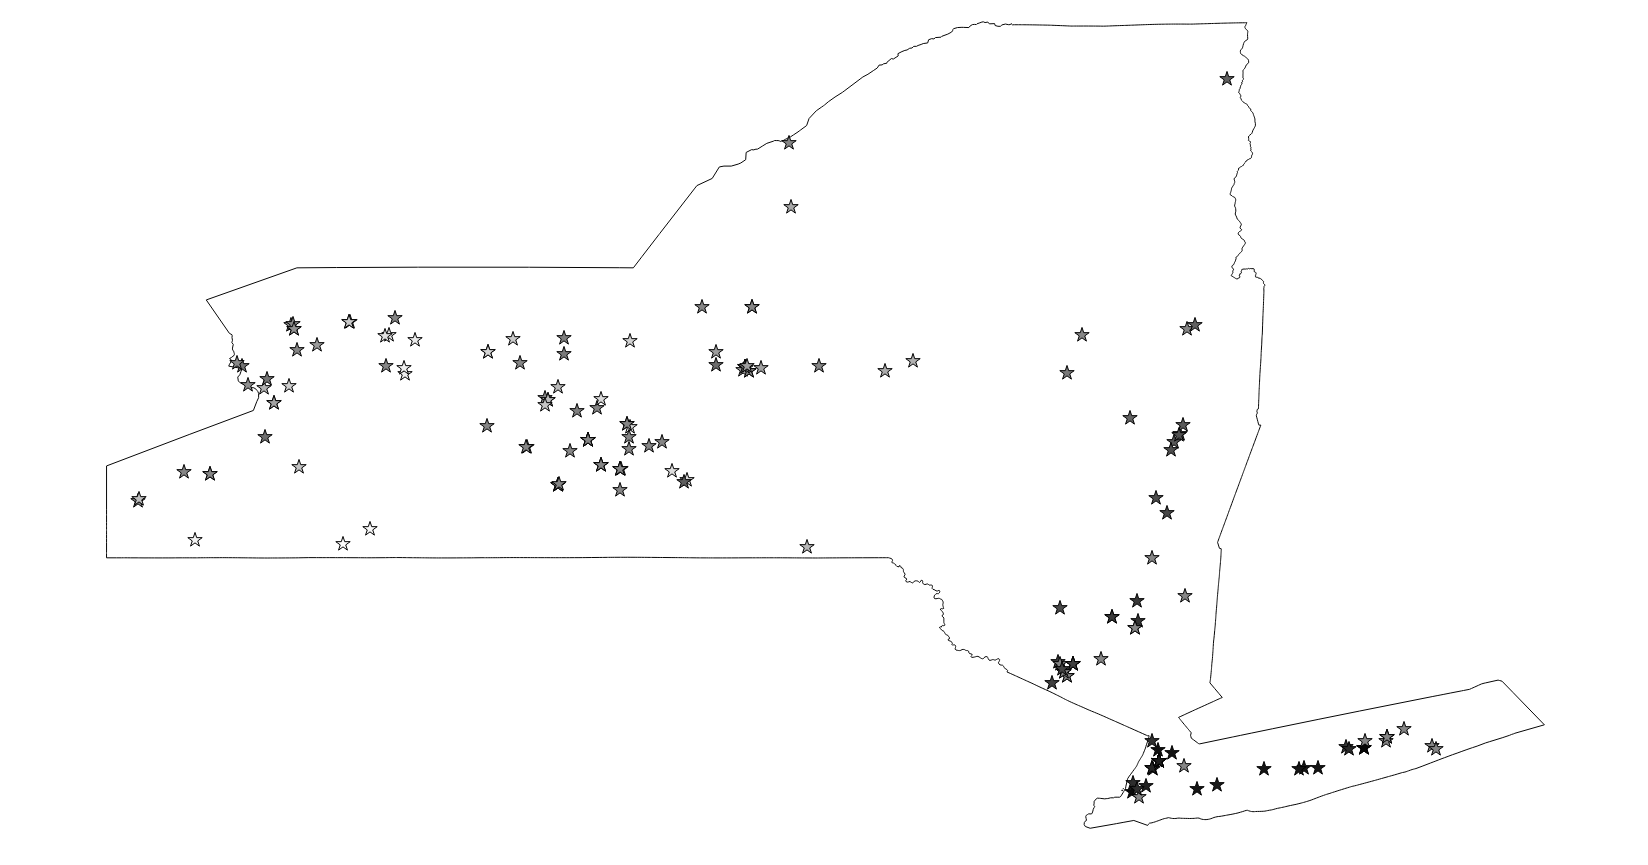
\includegraphics[scale=.50]{procs_243_66}
\caption{This figure compares the difference in prices between cherries and cabbages at the intermediaries. I chose cabbages because the result of the linear program was most different for this band. The stars represent the dealers. Darker means cherry prices were greater. Lighter means cabbage prices were greater.}
\label{fig:procs_243_66}
\end{framed}
\end{sidewaysfigure}

\begin{sidewaysfigure}[!htb]
\centering
\begin{framed}
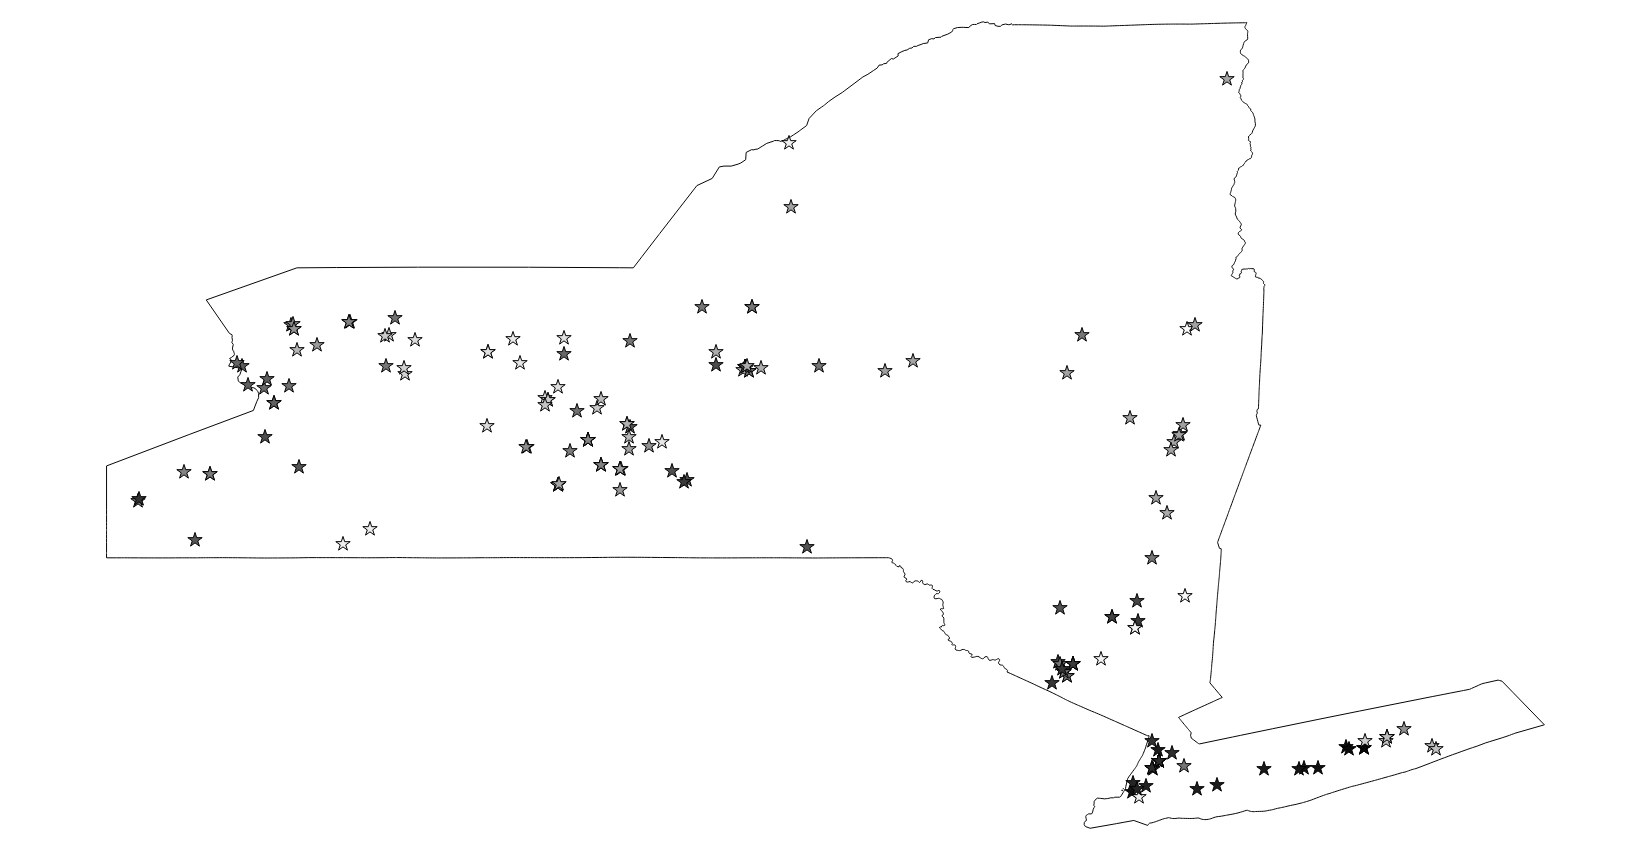
\includegraphics[scale=.50]{procs_243_69}
\caption{This figure compares the difference in prices between grapes and cabbages at the intermediaries. I chose cabbages because the result of the linear program was most different for this band. The stars represent the dealers. Darker means grape prices were greater. Lighter means cabbage prices were greater.}
\label{fig:procs_243_69}
\end{framed}
\end{sidewaysfigure}

\begin{sidewaysfigure}[!htb]
\centering
\begin{framed}
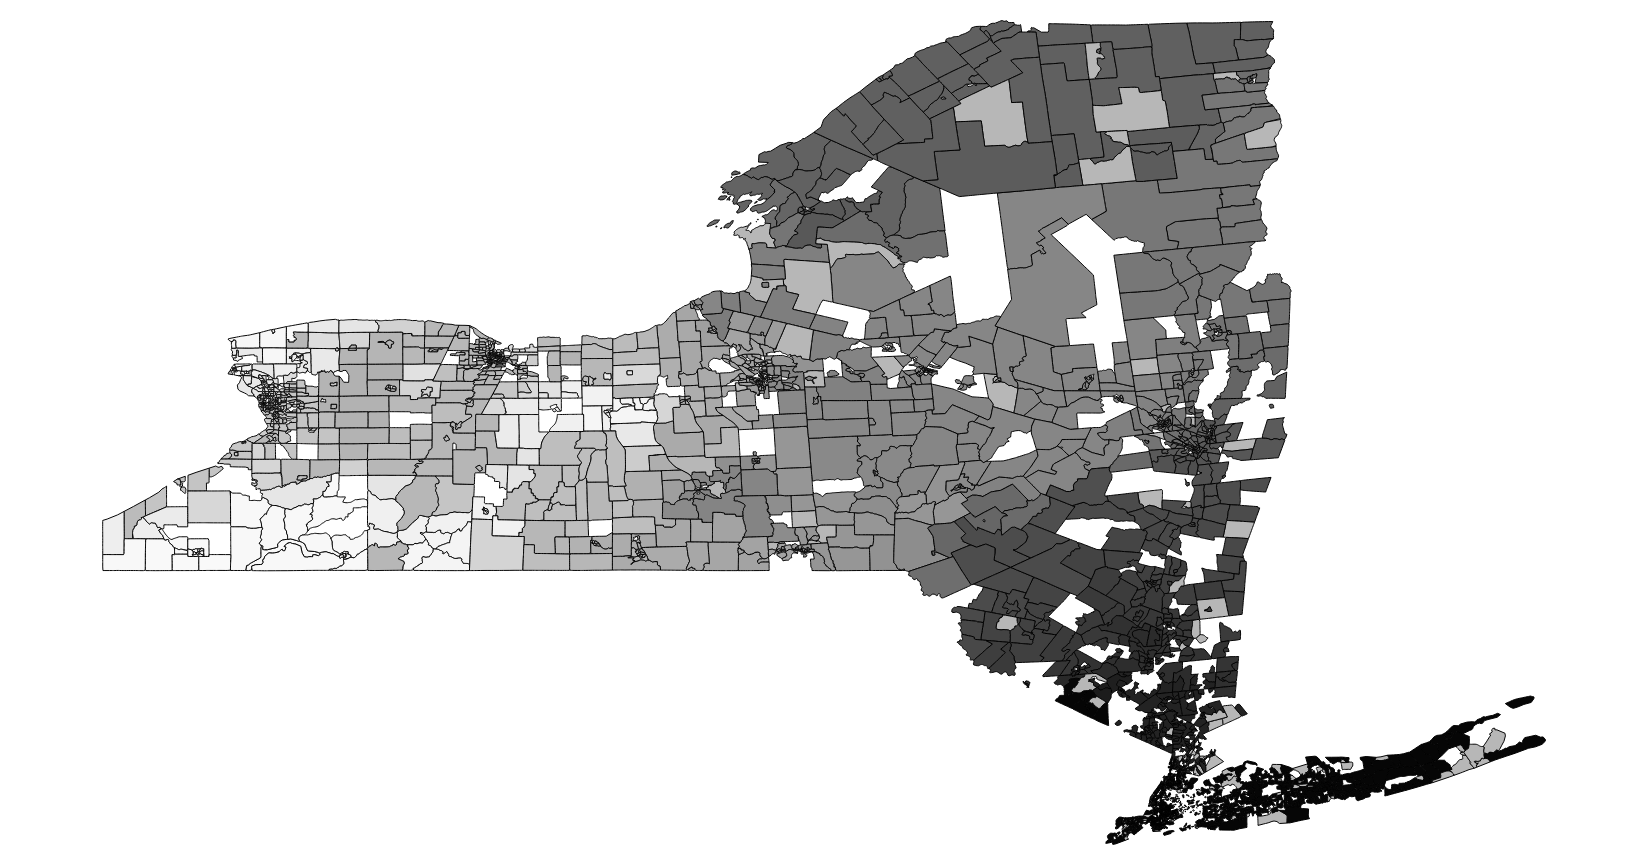
\includegraphics[scale=.50]{stores_243_49}
\caption{This figure compares the difference in prices between onions and cabbages at the census tracts. I chose cabbages because the result of the linear program was most different for this band. The stars represent the dealers. Darker means onion prices were greater. Lighter means cabbage prices were greater.}
\label{fig:stores_243_49}
\end{framed}
\end{sidewaysfigure}

\begin{sidewaysfigure}[!htb]
\centering
\begin{framed}
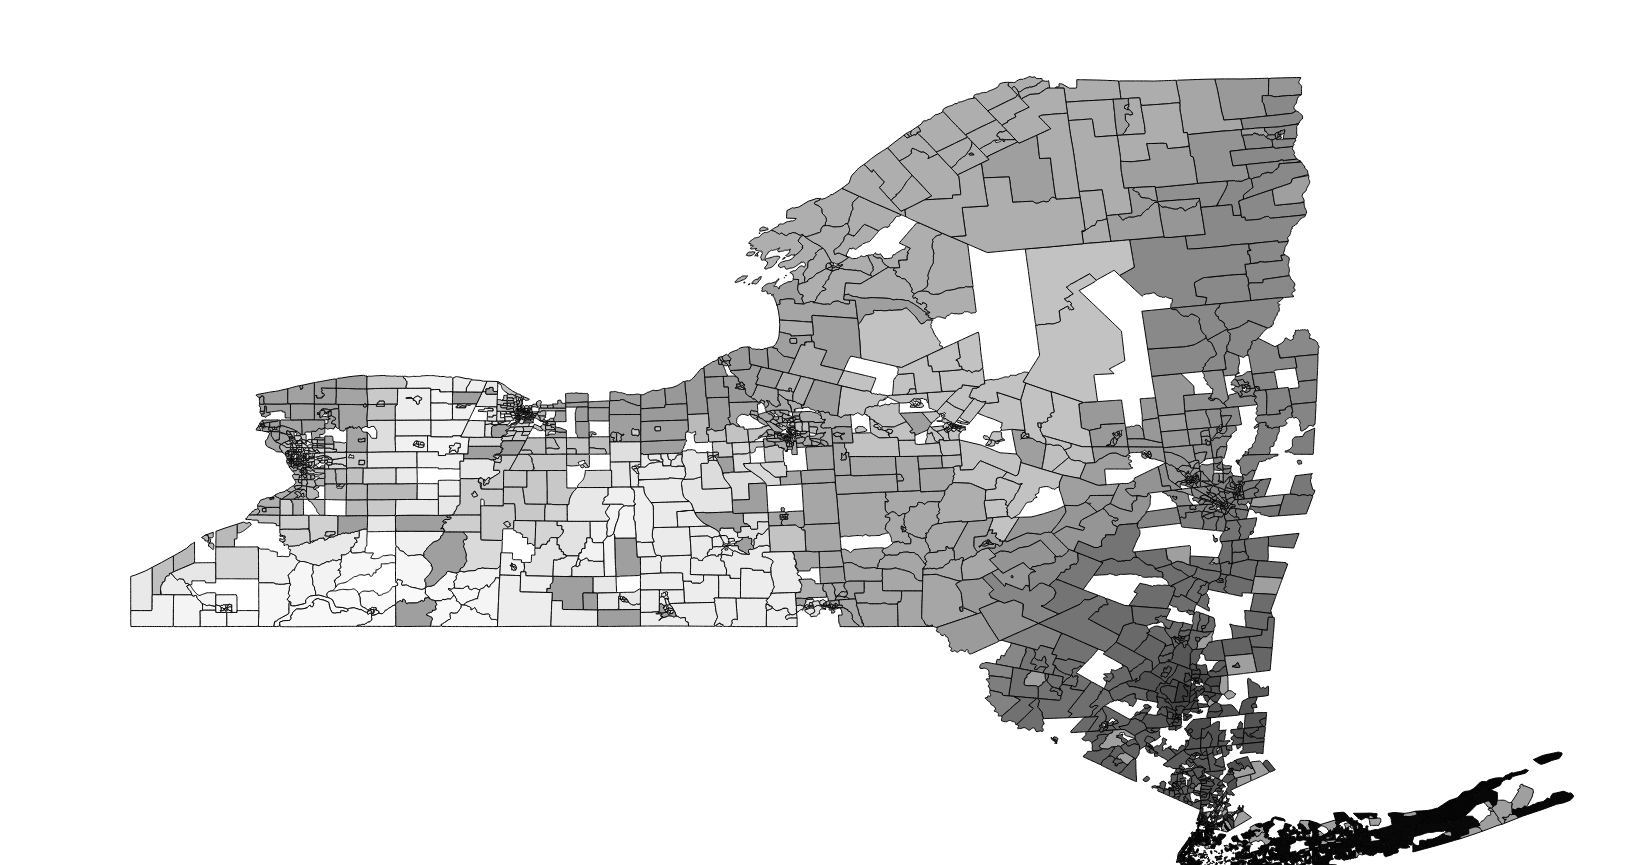
\includegraphics[scale=.50]{stores_243_66}
\caption{This figure compares the difference in prices between cherries and cabbages at the census tracts. I chose cabbages because the result of the linear program was most different for this band. The stars represent the dealers. Darker means cherry prices were greater. Lighter means cabbage prices were greater.}
\label{fig:stores_243_66}
\end{framed}
\end{sidewaysfigure}

\begin{sidewaysfigure}[!htb]
\centering
\begin{framed}
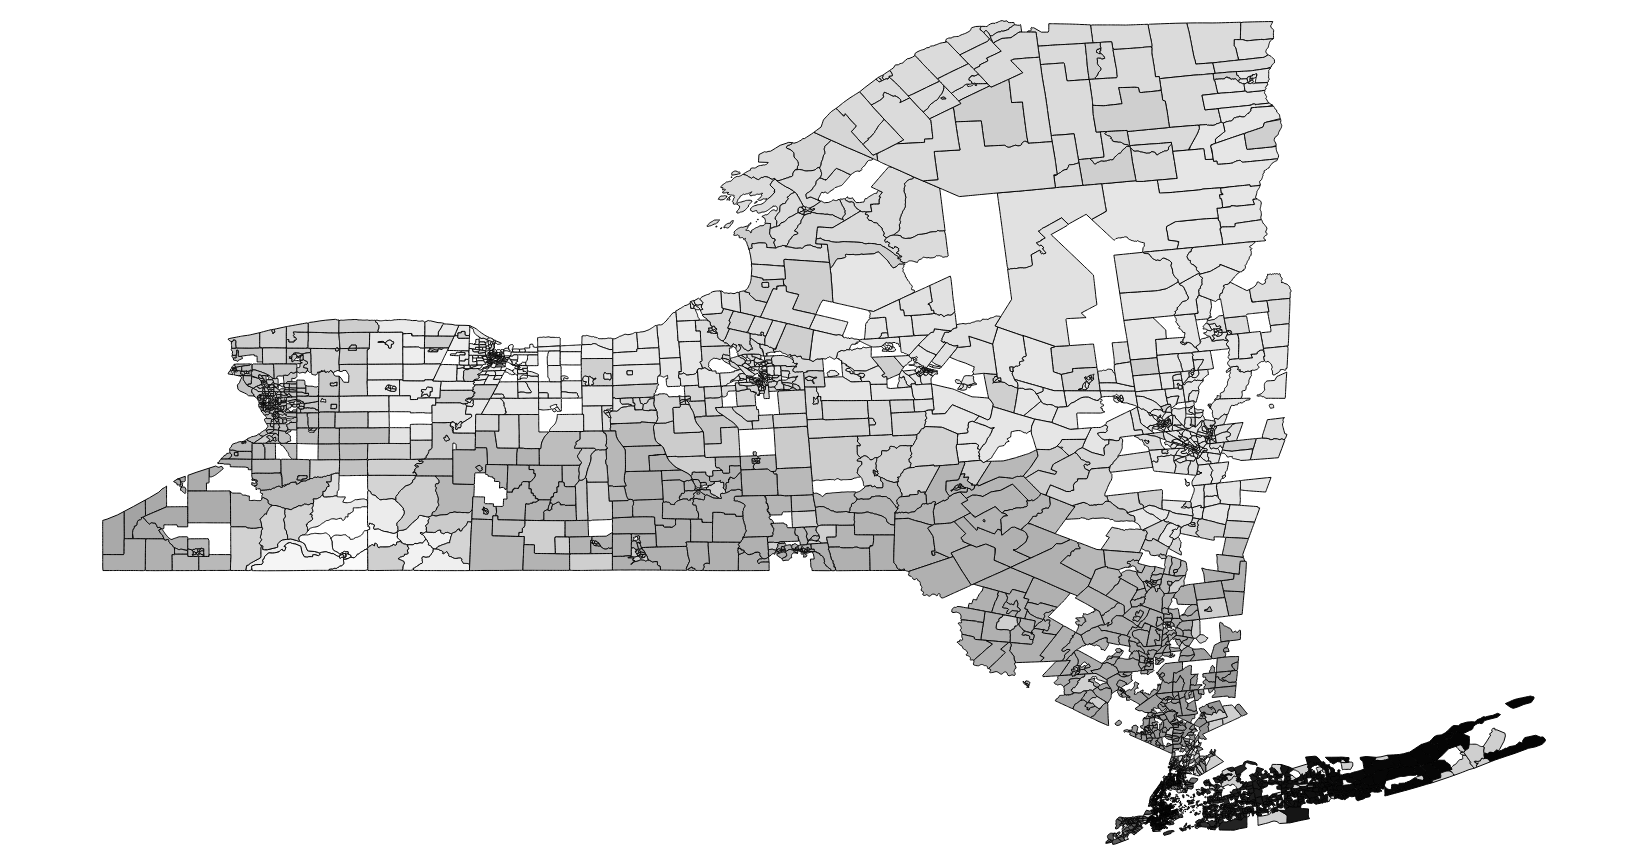
\includegraphics[scale=.50]{stores_243_69}
\caption{This figure compares the difference in prices between grapes and cabbages at the census tracts. I chose cabbages because the result of the linear program was most different for this band. The stars represent the dealers. Darker means grape prices were greater. Lighter means cabbage prices were greater.}
\label{fig:stores_243_69}
\end{framed}
\end{sidewaysfigure}


\end{document}